%********************************************%
%*       Generated from PreTeXt source      *%
%*       on 2021-09-25T15:48:38-04:00       *%
%*   A recent stable commit (2020-08-09):   *%
%* 98f21740783f166a773df4dc83cab5293ab63a4a *%
%*                                          *%
%*         https://pretextbook.org          *%
%*                                          *%
%********************************************%
%% We elect to always write snapshot output into <job>.dep file
\RequirePackage{snapshot}
\documentclass[oneside,10pt,]{book}
%% Custom Preamble Entries, early (use latex.preamble.early)
%% Default LaTeX packages
%%   1.  always employed (or nearly so) for some purpose, or
%%   2.  a stylewriter may assume their presence
\usepackage{geometry}
%% Some aspects of the preamble are conditional,
%% the LaTeX engine is one such determinant
\usepackage{ifthen}
%% etoolbox has a variety of modern conveniences
\usepackage{etoolbox}
\usepackage{ifxetex,ifluatex}
%% Raster graphics inclusion
\usepackage{graphicx}
%% Color support, xcolor package
%% Always loaded, for: add/delete text, author tools
%% Here, since tcolorbox loads tikz, and tikz loads xcolor
\PassOptionsToPackage{usenames,dvipsnames,svgnames,table}{xcolor}
\usepackage{xcolor}
%% begin: defined colors, via xcolor package, for styling
%% end: defined colors, via xcolor package, for styling
%% Colored boxes, and much more, though mostly styling
%% skins library provides "enhanced" skin, employing tikzpicture
%% boxes may be configured as "breakable" or "unbreakable"
%% "raster" controls grids of boxes, aka side-by-side
\usepackage{tcolorbox}
\tcbuselibrary{skins}
\tcbuselibrary{breakable}
\tcbuselibrary{raster}
%% We load some "stock" tcolorbox styles that we use a lot
%% Placement here is provisional, there will be some color work also
%% First, black on white, no border, transparent, but no assumption about titles
\tcbset{ bwminimalstyle/.style={size=minimal, boxrule=-0.3pt, frame empty,
colback=white, colbacktitle=white, coltitle=black, opacityfill=0.0} }
%% Second, bold title, run-in to text/paragraph/heading
%% Space afterwards will be controlled by environment,
%% independent of constructions of the tcb title
%% Places \blocktitlefont onto many block titles
\tcbset{ runintitlestyle/.style={fonttitle=\blocktitlefont\upshape\bfseries, attach title to upper} }
%% Spacing prior to each exercise, anywhere
\tcbset{ exercisespacingstyle/.style={before skip={1.5ex plus 0.5ex}} }
%% Spacing prior to each block
\tcbset{ blockspacingstyle/.style={before skip={2.0ex plus 0.5ex}} }
%% xparse allows the construction of more robust commands,
%% this is a necessity for isolating styling and behavior
%% The tcolorbox library of the same name loads the base library
\tcbuselibrary{xparse}
%% Hyperref should be here, but likes to be loaded late
%%
%% Inline math delimiters, \(, \), need to be robust
%% 2016-01-31:  latexrelease.sty  supersedes  fixltx2e.sty
%% If  latexrelease.sty  exists, bugfix is in kernel
%% If not, bugfix is in  fixltx2e.sty
%% See:  https://tug.org/TUGboat/tb36-3/tb114ltnews22.pdf
%% and read "Fewer fragile commands" in distribution's  latexchanges.pdf
\IfFileExists{latexrelease.sty}{}{\usepackage{fixltx2e}}
%% shorter subnumbers in some side-by-side require manipulations
\usepackage{xstring}
%% Text height identically 9 inches, text width varies on point size
%% See Bringhurst 2.1.1 on measure for recommendations
%% 75 characters per line (count spaces, punctuation) is target
%% which is the upper limit of Bringhurst's recommendations
\geometry{letterpaper,total={340pt,9.0in}}
%% Custom Page Layout Adjustments (use latex.geometry)
\geometry{letterpaper,left=1.5in,right=1in}
%% This LaTeX file may be compiled with pdflatex, xelatex, or lualatex executables
%% LuaTeX is not explicitly supported, but we do accept additions from knowledgeable users
%% The conditional below provides  pdflatex  specific configuration last
%% begin: engine-specific capabilities
\ifthenelse{\boolean{xetex} \or \boolean{luatex}}{%
%% begin: xelatex and lualatex-specific default configuration
\ifxetex\usepackage{xltxtra}\fi
%% realscripts is the only part of xltxtra relevant to lualatex 
\ifluatex\usepackage{realscripts}\fi
%% end:   xelatex and lualatex-specific default configuration
}{
%% begin: pdflatex-specific default configuration
%% We assume a PreTeXt XML source file may have Unicode characters
%% and so we ask LaTeX to parse a UTF-8 encoded file
%% This may work well for accented characters in Western language,
%% but not with Greek, Asian languages, etc.
%% When this is not good enough, switch to the  xelatex  engine
%% where Unicode is better supported (encouraged, even)
\usepackage[utf8]{inputenc}
%% end: pdflatex-specific default configuration
}
%% end:   engine-specific capabilities
%%
%% Fonts.  Conditional on LaTex engine employed.
%% Default Text Font: The Latin Modern fonts are
%% "enhanced versions of the [original TeX] Computer Modern fonts."
%% We use them as the default text font for PreTeXt output.
%% Automatic Font Control
%% Portions of a document, are, or may, be affected by defined commands
%% These are perhaps more flexible when using  xelatex  rather than  pdflatex
%% The following definitions are meant to be re-defined in a style, using \renewcommand
%% They are scoped when employed (in a TeX group), and so should not be defined with an argument
\newcommand{\divisionfont}{\relax}
\newcommand{\blocktitlefont}{\relax}
\newcommand{\contentsfont}{\relax}
\newcommand{\pagefont}{\relax}
\newcommand{\tabularfont}{\relax}
\newcommand{\xreffont}{\relax}
\newcommand{\titlepagefont}{\relax}
%%
\ifthenelse{\boolean{xetex} \or \boolean{luatex}}{%
%% begin: font setup and configuration for use with xelatex
%% Generally, xelatex is necessary for non-Western fonts
%% fontspec package provides extensive control of system fonts,
%% meaning *.otf (OpenType), and apparently *.ttf (TrueType)
%% that live *outside* your TeX/MF tree, and are controlled by your *system*
%% (it is possible that a TeX distribution will place fonts in a system location)
%%
%% The fontspec package is the best vehicle for using different fonts in  xelatex
%% So we load it always, no matter what a publisher or style might want
%%
\usepackage{fontspec}
%%
%% begin: xelatex main font ("font-xelatex-main" template)
%% Latin Modern Roman is the default font for xelatex and so is loaded with a TU encoding
%% *in the format* so we can't touch it, only perhaps adjust it later
%% in one of two ways (then known by NFSS names such as "lmr")
%% (1) via NFSS with font family names such as "lmr" and "lmss"
%% (2) via fontspec with commands like \setmainfont{Latin Modern Roman}
%% The latter requires the font to be known at the system-level by its font name,
%% but will give access to OTF font features through optional arguments
%% https://tex.stackexchange.com/questions/470008/
%% where-and-how-does-fontspec-sty-specify-the-default-font-latin-modern-roman
%% http://tex.stackexchange.com/questions/115321
%% /how-to-optimize-latin-modern-font-with-xelatex
%%
%% end:   xelatex main font ("font-xelatex-main" template)
%% begin: xelatex mono font ("font-xelatex-mono" template)
%% (conditional on non-trivial uses being present in source)
%% end:   xelatex mono font ("font-xelatex-mono" template)
%% begin: xelatex font adjustments ("font-xelatex-style" template)
%% end:   xelatex font adjustments ("font-xelatex-style" template)
%%
%% Extensive support for other languages
\usepackage{polyglossia}
%% Set main/default language based on pretext/@xml:lang value
%% document language code is "en-US", US English
%% usmax variant has extra hypenation
\setmainlanguage[variant=usmax]{english}
%% Enable secondary languages based on discovery of @xml:lang values
%% Enable fonts/scripts based on discovery of @xml:lang values
%% Western languages should be ably covered by Latin Modern Roman
%% end:   font setup and configuration for use with xelatex
}{%
%% begin: font setup and configuration for use with pdflatex
%% begin: pdflatex main font ("font-pdflatex-main" template)
\usepackage{lmodern}
\usepackage[T1]{fontenc}
%% end:   pdflatex main font ("font-pdflatex-main" template)
%% begin: pdflatex mono font ("font-pdflatex-mono" template)
%% (conditional on non-trivial uses being present in source)
%% end:   pdflatex mono font ("font-pdflatex-mono" template)
%% begin: pdflatex font adjustments ("font-pdflatex-style" template)
%% end:   pdflatex font adjustments ("font-pdflatex-style" template)
%% end:   font setup and configuration for use with pdflatex
}
%% Micromanage spacing, etc.  The named "microtype-options"
%% template may be employed to fine-tune package behavior
\usepackage{microtype}
%% Symbols, align environment, commutative diagrams, bracket-matrix
\usepackage{amsmath}
\usepackage{amscd}
\usepackage{amssymb}
%% allow page breaks within display mathematics anywhere
%% level 4 is maximally permissive
%% this is exactly the opposite of AMSmath package philosophy
%% there are per-display, and per-equation options to control this
%% split, aligned, gathered, and alignedat are not affected
\allowdisplaybreaks[4]
%% allow more columns to a matrix
%% can make this even bigger by overriding with  latex.preamble.late  processing option
\setcounter{MaxMatrixCols}{30}
%%
%%
%% Division Titles, and Page Headers/Footers
%% titlesec package, loading "titleps" package cooperatively
%% See code comments about the necessity and purpose of "explicit" option.
%% The "newparttoc" option causes a consistent entry for parts in the ToC 
%% file, but it is only effective if there is a \titleformat for \part.
%% "pagestyles" loads the  titleps  package cooperatively.
\usepackage[explicit, newparttoc, pagestyles]{titlesec}
%% The companion titletoc package for the ToC.
\usepackage{titletoc}
%% Fixes a bug with transition from chapters to appendices in a "book"
%% See generating XSL code for more details about necessity
\newtitlemark{\chaptertitlename}
%% begin: customizations of page styles via the modal "titleps-style" template
%% Designed to use commands from the LaTeX "titleps" package
%% Plain pages should have the same font for page numbers
\renewpagestyle{plain}{%
\setfoot{}{\pagefont\thepage}{}%
}%
%% Single pages as in default LaTeX
\renewpagestyle{headings}{%
\sethead{\pagefont\slshape\MakeUppercase{\ifthechapter{\chaptertitlename\space\thechapter.\space}{}\chaptertitle}}{}{\pagefont\thepage}%
}%
\pagestyle{headings}
%% end: customizations of page styles via the modal "titleps-style" template
%%
%% Create globally-available macros to be provided for style writers
%% These are redefined for each occurence of each division
\newcommand{\divisionnameptx}{\relax}%
\newcommand{\titleptx}{\relax}%
\newcommand{\subtitleptx}{\relax}%
\newcommand{\shortitleptx}{\relax}%
\newcommand{\authorsptx}{\relax}%
\newcommand{\epigraphptx}{\relax}%
%% Create environments for possible occurences of each division
%% Environment for a PTX "preface" at the level of a LaTeX "chapter"
\NewDocumentEnvironment{preface}{mmmmmm}
{%
\renewcommand{\divisionnameptx}{Preface}%
\renewcommand{\titleptx}{#1}%
\renewcommand{\subtitleptx}{#2}%
\renewcommand{\shortitleptx}{#3}%
\renewcommand{\authorsptx}{#4}%
\renewcommand{\epigraphptx}{#5}%
\chapter*{#1}%
\addcontentsline{toc}{chapter}{#3}
\label{#6}%
}{}%
%% Environment for a PTX "chapter" at the level of a LaTeX "chapter"
\NewDocumentEnvironment{chapterptx}{mmmmmm}
{%
\renewcommand{\divisionnameptx}{Chapter}%
\renewcommand{\titleptx}{#1}%
\renewcommand{\subtitleptx}{#2}%
\renewcommand{\shortitleptx}{#3}%
\renewcommand{\authorsptx}{#4}%
\renewcommand{\epigraphptx}{#5}%
\chapter[{#3}]{#1}%
\label{#6}%
}{}%
%% Environment for a PTX "section" at the level of a LaTeX "section"
\NewDocumentEnvironment{sectionptx}{mmmmmm}
{%
\renewcommand{\divisionnameptx}{Section}%
\renewcommand{\titleptx}{#1}%
\renewcommand{\subtitleptx}{#2}%
\renewcommand{\shortitleptx}{#3}%
\renewcommand{\authorsptx}{#4}%
\renewcommand{\epigraphptx}{#5}%
\section[{#3}]{#1}%
\label{#6}%
}{}%
%% Environment for a PTX "subsection" at the level of a LaTeX "subsection"
\NewDocumentEnvironment{subsectionptx}{mmmmmm}
{%
\renewcommand{\divisionnameptx}{Subsection}%
\renewcommand{\titleptx}{#1}%
\renewcommand{\subtitleptx}{#2}%
\renewcommand{\shortitleptx}{#3}%
\renewcommand{\authorsptx}{#4}%
\renewcommand{\epigraphptx}{#5}%
\subsection[{#3}]{#1}%
\label{#6}%
}{}%
%% Environment for a PTX "subsubsection" at the level of a LaTeX "subsubsection"
\NewDocumentEnvironment{subsubsectionptx}{mmmmmm}
{%
\renewcommand{\divisionnameptx}{Subsubsection}%
\renewcommand{\titleptx}{#1}%
\renewcommand{\subtitleptx}{#2}%
\renewcommand{\shortitleptx}{#3}%
\renewcommand{\authorsptx}{#4}%
\renewcommand{\epigraphptx}{#5}%
\subsubsection[{#3}]{#1}%
\label{#6}%
}{}%
%% Environment for a PTX "exercises" at the level of a LaTeX "subsection"
\NewDocumentEnvironment{exercises-subsection}{mmmmmm}
{%
\renewcommand{\divisionnameptx}{Exercises}%
\renewcommand{\titleptx}{#1}%
\renewcommand{\subtitleptx}{#2}%
\renewcommand{\shortitleptx}{#3}%
\renewcommand{\authorsptx}{#4}%
\renewcommand{\epigraphptx}{#5}%
\subsection[{#3}]{#1}%
\label{#6}%
}{}%
%% Environment for a PTX "exercises" at the level of a LaTeX "subsection"
\NewDocumentEnvironment{exercises-subsection-numberless}{mmmmmm}
{%
\renewcommand{\divisionnameptx}{Exercises}%
\renewcommand{\titleptx}{#1}%
\renewcommand{\subtitleptx}{#2}%
\renewcommand{\shortitleptx}{#3}%
\renewcommand{\authorsptx}{#4}%
\renewcommand{\epigraphptx}{#5}%
\subsection*{#1}%
\addcontentsline{toc}{subsection}{#3}
\label{#6}%
}{}%
%%
%% Styles for six traditional LaTeX divisions
\titleformat{\part}[display]
{\divisionfont\Huge\bfseries\centering}{\divisionnameptx\space\thepart}{30pt}{\Huge#1}
[{\Large\centering\authorsptx}]
\titleformat{\chapter}[display]
{\divisionfont\huge\bfseries}{\divisionnameptx\space\thechapter}{20pt}{\Huge#1}
[{\Large\authorsptx}]
\titleformat{name=\chapter,numberless}[display]
{\divisionfont\huge\bfseries}{}{0pt}{#1}
[{\Large\authorsptx}]
\titlespacing*{\chapter}{0pt}{50pt}{40pt}
\titleformat{\section}[hang]
{\divisionfont\Large\bfseries}{\thesection}{1ex}{#1}
[{\large\authorsptx}]
\titleformat{name=\section,numberless}[block]
{\divisionfont\Large\bfseries}{}{0pt}{#1}
[{\large\authorsptx}]
\titlespacing*{\section}{0pt}{3.5ex plus 1ex minus .2ex}{2.3ex plus .2ex}
\titleformat{\subsection}[hang]
{\divisionfont\large\bfseries}{\thesubsection}{1ex}{#1}
[{\normalsize\authorsptx}]
\titleformat{name=\subsection,numberless}[block]
{\divisionfont\large\bfseries}{}{0pt}{#1}
[{\normalsize\authorsptx}]
\titlespacing*{\subsection}{0pt}{3.25ex plus 1ex minus .2ex}{1.5ex plus .2ex}
\titleformat{\subsubsection}[hang]
{\divisionfont\normalsize\bfseries}{\thesubsubsection}{1em}{#1}
[{\small\authorsptx}]
\titleformat{name=\subsubsection,numberless}[block]
{\divisionfont\normalsize\bfseries}{}{0pt}{#1}
[{\normalsize\authorsptx}]
\titlespacing*{\subsubsection}{0pt}{3.25ex plus 1ex minus .2ex}{1.5ex plus .2ex}
\titleformat{\paragraph}[hang]
{\divisionfont\normalsize\bfseries}{\theparagraph}{1em}{#1}
[{\small\authorsptx}]
\titleformat{name=\paragraph,numberless}[block]
{\divisionfont\normalsize\bfseries}{}{0pt}{#1}
[{\normalsize\authorsptx}]
\titlespacing*{\paragraph}{0pt}{3.25ex plus 1ex minus .2ex}{1.5em}
%%
%% Styles for five traditional LaTeX divisions
\titlecontents{part}%
[0pt]{\contentsmargin{0em}\addvspace{1pc}\contentsfont\bfseries}%
{\Large\thecontentslabel\enspace}{\Large}%
{}%
[\addvspace{.5pc}]%
\titlecontents{chapter}%
[0pt]{\contentsmargin{0em}\addvspace{1pc}\contentsfont\bfseries}%
{\large\thecontentslabel\enspace}{\large}%
{\hfill\bfseries\thecontentspage}%
[\addvspace{.5pc}]%
\dottedcontents{section}[3.8em]{\contentsfont}{2.3em}{1pc}%
\dottedcontents{subsection}[6.1em]{\contentsfont}{3.2em}{1pc}%
\dottedcontents{subsubsection}[9.3em]{\contentsfont}{4.3em}{1pc}%
%%
%% Begin: Semantic Macros
%% To preserve meaning in a LaTeX file
%%
%% \mono macro for content of "c", "cd", "tag", etc elements
%% Also used automatically in other constructions
%% Simply an alias for \texttt
%% Always defined, even if there is no need, or if a specific tt font is not loaded
\newcommand{\mono}[1]{\texttt{#1}}
%%
%% Following semantic macros are only defined here if their
%% use is required only in this specific document
%%
%% Used for inline definitions of terms
\newcommand{\terminology}[1]{\textbf{#1}}
%% Used for fillin answer blank
%% Argument is length in em
%% Length may compress for output to fit in one line
\newcommand{\fillin}[1]{\leavevmode\leaders\vrule height -1.2pt depth 1.5pt \hskip #1em minus #1em \null}
%% End: Semantic Macros
%% Divisional exercises (and worksheet) as LaTeX environments
%% Third argument is option for extra workspace in worksheets
%% Hanging indent occupies a 5ex width slot prior to left margin
%% Experimentally this seems just barely sufficient for a bold "888."
%% Division exercises, not in exercise group
\tcbset{ divisionexercisestyle/.style={bwminimalstyle, runintitlestyle, exercisespacingstyle, left=5ex, breakable, parbox=false } }
\newtcolorbox{divisionexercise}[4]{divisionexercisestyle, before title={\hspace{-5ex}\makebox[5ex][l]{#1.}}, title={\notblank{#2}{#2\space}{}}, phantom={\hypertarget{#4}{}}, after={\notblank{#3}{\newline\rule{\workspacestrutwidth}{#3}\newline\vfill}{}}}
%% Division exercises, in exercise group with columns
\tcbset{ divisionexerciseegcolstyle/.style={bwminimalstyle, runintitlestyle, exercisespacingstyle, left=5ex, halign=flush left, unbreakable, parbox=false } }
\newtcolorbox{divisionexerciseegcol}[4]{divisionexerciseegcolstyle, before title={\hspace{-5ex}\makebox[5ex][l]{#1.}}, title={\notblank{#2}{#2\space}{}}, phantom={\hypertarget{#4}{}}, after={\notblank{#3}{\newline\rule{\workspacestrutwidth}{#3}\newline\vfill}{}}}
%% Localize LaTeX supplied names (possibly none)
\renewcommand*{\chaptername}{Chapter}
%% Equation Numbering
%% Controlled by  numbering.equations.level  processing parameter
%% No adjustment here implies document-wide numbering
\numberwithin{equation}{section}
%% "tcolorbox" environment for a single image, occupying entire \linewidth
%% arguments are left-margin, width, right-margin, as multiples of
%% \linewidth, and are guaranteed to be positive and sum to 1.0
\tcbset{ imagestyle/.style={bwminimalstyle} }
\NewTColorBox{image}{mmm}{imagestyle,left skip=#1\linewidth,width=#2\linewidth}
%% For improved tables
\usepackage{array}
%% Some extra height on each row is desirable, especially with horizontal rules
%% Increment determined experimentally
\setlength{\extrarowheight}{0.2ex}
%% Define variable thickness horizontal rules, full and partial
%% Thicknesses are 0.03, 0.05, 0.08 in the  booktabs  package
\newcommand{\hrulethin}  {\noalign{\hrule height 0.04em}}
\newcommand{\hrulemedium}{\noalign{\hrule height 0.07em}}
\newcommand{\hrulethick} {\noalign{\hrule height 0.11em}}
%% We preserve a copy of the \setlength package before other
%% packages (extpfeil) get a chance to load packages that redefine it
\let\oldsetlength\setlength
\newlength{\Oldarrayrulewidth}
\newcommand{\crulethin}[1]%
{\noalign{\global\oldsetlength{\Oldarrayrulewidth}{\arrayrulewidth}}%
\noalign{\global\oldsetlength{\arrayrulewidth}{0.04em}}\cline{#1}%
\noalign{\global\oldsetlength{\arrayrulewidth}{\Oldarrayrulewidth}}}%
\newcommand{\crulemedium}[1]%
{\noalign{\global\oldsetlength{\Oldarrayrulewidth}{\arrayrulewidth}}%
\noalign{\global\oldsetlength{\arrayrulewidth}{0.07em}}\cline{#1}%
\noalign{\global\oldsetlength{\arrayrulewidth}{\Oldarrayrulewidth}}}
\newcommand{\crulethick}[1]%
{\noalign{\global\oldsetlength{\Oldarrayrulewidth}{\arrayrulewidth}}%
\noalign{\global\oldsetlength{\arrayrulewidth}{0.11em}}\cline{#1}%
\noalign{\global\oldsetlength{\arrayrulewidth}{\Oldarrayrulewidth}}}
%% Single letter column specifiers defined via array package
\newcolumntype{A}{!{\vrule width 0.04em}}
\newcolumntype{B}{!{\vrule width 0.07em}}
\newcolumntype{C}{!{\vrule width 0.11em}}
%% tcolorbox to place tabular outside of a sidebyside
\tcbset{ tabularboxstyle/.style={bwminimalstyle,} }
\newtcolorbox{tabularbox}[3]{tabularboxstyle, left skip=#1\linewidth, width=#2\linewidth,}
\newcommand{\tablecelllines}[3]%
{\begin{tabular}[#2]{@{}#1@{}}#3\end{tabular}}
%% Multiple column, column-major lists
\usepackage{multicol}
%% More flexible list management, esp. for references
%% But also for specifying labels (i.e. custom order) on nested lists
\usepackage{enumitem}
%% Indented groups of "exercise" within an "exercises" division
%% Lengths control the indentation (always) and gaps (multi-column)
\newlength{\egindent}\setlength{\egindent}{0.05\linewidth}
\newlength{\exggap}\setlength{\exggap}{0.05\linewidth}
%% An exercise group with multiple columns is a tcbraster.
%% If the contained exercises are explicitly unbreakable,
%% the raster should break at rows for page breaks.
%% The number of columns is a parameter, passed to tcbraster.
\tcbset{ exgroupcolstyle/.style={raster equal height=rows, raster left skip=\egindent, raster column skip=\exggap} }
\NewDocumentEnvironment{exercisegroupcol}{m}
{\begin{tcbraster}[exgroupcolstyle,raster columns=#1]}{\end{tcbraster}}
%% hyperref driver does not need to be specified, it will be detected
%% Footnote marks in tcolorbox have broken linking under
%% hyperref, so it is necessary to turn off all linking
%% It *must* be given as a package option, not with \hypersetup
\usepackage[hyperfootnotes=false]{hyperref}
%% Hyperlinking active in electronic PDFs, all links solid and blue
\hypersetup{colorlinks=true,linkcolor=blue,citecolor=blue,filecolor=blue,urlcolor=blue}
\hypersetup{pdftitle={Test chapters}}
%% If you manually remove hyperref, leave in this next command
%% This will allow LaTeX compilation, employing this no-op command
\providecommand\phantomsection{}
%% Division Numbering: Chapters, Sections, Subsections, etc
%% Division numbers may be turned off at some level ("depth")
%% A section *always* has depth 1, contrary to us counting from the document root
%% The latex default is 3.  If a larger number is present here, then
%% removing this command may make some cross-references ambiguous
%% The precursor variable $numbering-maxlevel is checked for consistency in the common XSL file
\setcounter{secnumdepth}{1}
%%
%% AMS "proof" environment is no longer used, but we leave previously
%% implemented \qedhere in place, should the LaTeX be recycled
\newcommand{\qedhere}{\relax}
%%
%% A faux tcolorbox whose only purpose is to provide common numbering
%% facilities for most blocks (possibly not projects, 2D displays)
%% Controlled by  numbering.theorems.level  processing parameter
\newtcolorbox[auto counter, number within=chapter]{block}{}
%%
%% This document is set to number PROJECT-LIKE on a separate numbering scheme
%% So, a faux tcolorbox whose only purpose is to provide this numbering
%% Controlled by  numbering.projects.level  processing parameter
\newtcolorbox[auto counter, number within=chapter]{project-distinct}{}
%% A faux tcolorbox whose only purpose is to provide common numbering
%% facilities for 2D displays which are subnumbered as part of a "sidebyside"
\makeatletter
\newtcolorbox[auto counter, number within=tcb@cnt@block, number freestyle={\noexpand\thetcb@cnt@block(\noexpand\alph{\tcbcounter})}]{subdisplay}{}
\makeatother
%%
%% tcolorbox, with styles, for REMARK-LIKE
%%
%% note: fairly simple numbered block/structure
\tcbset{ notestyle/.style={bwminimalstyle, runintitlestyle, blockspacingstyle, after title={\space}, } }
\newtcolorbox[use counter from=block]{note}[2]{title={{Note~\thetcbcounter\notblank{#1}{\space\space#1}{}}}, phantomlabel={#2}, breakable, parbox=false, after={\par}, notestyle, }
%%
%% tcolorbox, with styles, for COMPUTATION-LIKE
%%
%% technology: fairly simple numbered block/structure
\tcbset{ technologystyle/.style={bwminimalstyle, runintitlestyle, blockspacingstyle, after title={\space}, } }
\newtcolorbox[use counter from=block]{technology}[2]{title={{Technology~\thetcbcounter\notblank{#1}{\space\space#1}{}}}, phantomlabel={#2}, breakable, parbox=false, after={\par}, technologystyle, }
%%
%% tcolorbox, with styles, for EXAMPLE-LIKE
%%
%% example: fairly simple numbered block/structure
\tcbset{ examplestyle/.style={enhanced, colback=white, colframe=black,
colbacktitle=blue!45!black, coltitle=white, boxed title style={sharp corners, frame hidden},
fonttitle=\bfseries, attach boxed title to top left={xshift=4mm,yshift=-3mm}, top=3mm,
} }
\newtcolorbox[use counter from=block]{example}[2]{title={{Example~\thetcbcounter\notblank{#1}{\space\space#1}{}}}, phantomlabel={#2}, breakable, parbox=false, after={\par}, examplestyle, }
%%
%% tcolorbox, with styles, for inline exercises
%%
%% inlineexercise: fairly simple numbered block/structure
\tcbset{ inlineexercisestyle/.style={enhanced, arc=2ex, colback=white, colframe=teal!75!black,
colbacktitle=white, coltitle=black, boxed title style={sharp corners, frame hidden},
fonttitle=\bfseries, attach boxed title to top left={xshift=4mm,yshift=-3mm}, top=3mm,
} }
\newtcolorbox[use counter from=block]{inlineexercise}[2]{title={{Checkpoint~\thetcbcounter\notblank{#1}{\space\space#1}{}}}, phantomlabel={#2}, breakable, parbox=false, after={\par}, inlineexercisestyle, }
%%
%% tcolorbox, with styles, for PROJECT-LIKE
%%
%% investigation: fairly simple numbered block/structure
\tcbset{ investigationstyle/.style={enhanced, arc=2ex, colback=white, colframe=blue!10!black,
colbacktitle=white, coltitle=black, boxed title style={sharp corners, frame hidden},
fonttitle=\bfseries, attach boxed title to top left={xshift=4mm,yshift=-3mm}, top=3mm,
} }
\newtcolorbox[use counter from=project-distinct]{investigation}[2]{title={{Investigation~\thetcbcounter\notblank{#1}{\space\space#1}{}}}, phantomlabel={#2}, breakable, parbox=false, after={\par}, investigationstyle, }
%%
%% xparse environments for introductions and conclusions of divisions
%%
%% introduction: in a structured division
\NewDocumentEnvironment{introduction}{m}
{\notblank{#1}{\noindent\textbf{#1}\space}{}}{\par\medskip}
%%
%% tcolorbox, with styles, for miscellaneous environments
%%
%% assemblage: fairly simple un-numbered block/structure
\tcbset{ assemblagestyle/.style={enhanced, arc=2ex, colback=violet!5, colframe=violet!75!black,
colbacktitle=violet!45!white, coltitle=white, boxed title style={sharp corners, frame hidden},
fonttitle=\bfseries, attach boxed title to top left={xshift=4mm,yshift=-3mm}, top=3mm,
} }
\newtcolorbox{assemblage}[2]{title={\notblank{#1}{#1}{}}, phantomlabel={#2}, breakable, parbox=false, assemblagestyle}
%% Graphics Preamble Entries
\usepackage{tikz}
\usetikzlibrary{calc}
\usetikzlibrary{arrows}
\usetikzlibrary{decorations.pathreplacing}
\usetikzlibrary{patterns}
\usetikzlibrary{calc,intersections,through,backgrounds}
\usetikzlibrary{shapes.geometric}
%% If tikz has been loaded, replace ampersand with \amp macro
\ifdefined\tikzset
    \tikzset{ampersand replacement = \amp}
\fi
%% tcolorbox styles for sidebyside layout
\tcbset{ sbsstyle/.style={raster before skip=2.0ex, raster equal height=rows, raster force size=false} }
\tcbset{ sbspanelstyle/.style={bwminimalstyle, fonttitle=\blocktitlefont} }
%% Enviroments for side-by-side and components
%% Necessary to use \NewTColorBox for boxes of the panels
%% "newfloat" environment to squash page-breaks within a single sidebyside
%% "xparse" environment for entire sidebyside
\NewDocumentEnvironment{sidebyside}{mmmm}
  {\begin{tcbraster}
    [sbsstyle,raster columns=#1,
    raster left skip=#2\linewidth,raster right skip=#3\linewidth,raster column skip=#4\linewidth]}
  {\end{tcbraster}}
%% "tcolorbox" environment for a panel of sidebyside
\NewTColorBox{sbspanel}{mO{top}}{sbspanelstyle,width=#1\linewidth,valign=#2}
%% extpfeil package for certain extensible arrows,
%% as also provided by MathJax extension of the same name
%% NB: this package loads mtools, which loads calc, which redefines
%%     \setlength, so it can be removed if it seems to be in the 
%%     way and your math does not use:
%%     
%%     \xtwoheadrightarrow, \xtwoheadleftarrow, \xmapsto, \xlongequal, \xtofrom
%%     
%%     we have had to be extra careful with variable thickness
%%     lines in tables, and so also load this package late
\usepackage{extpfeil}
%% menukeys package says:
%%   Since menukeys uses catoptions, which does some heavy
%%   changes on key-value options, it is recommended to load
%%   menukeys as the last package (even after hyperref)!
\usepackage{menukeys}
\renewmenumacro{\keys}{shadowedroundedkeys}
\newcommand{\kbd}[1]{\keys{{#1}}}
%% Custom Preamble Entries, late (use latex.preamble.late)
%% Begin: Author-provided packages
%% (From  docinfo/latex-preamble/package  elements)
\usepackage{cancel}%% End: Author-provided packages
%% Begin: Author-provided macros
%% (From  docinfo/macros  element)
%% Plus three from MBX for XML characters
\newcommand\degree[0]{^{\circ}}
\newcommand\Ccancel[2][black]{\renewcommand\CancelColor{\color{#1}}\cancel{#2}}
\newcommand{\alert}[1]{\boldsymbol{\color{magenta}{#1}}}
\newcommand{\blert}[1]{\boldsymbol{\color{blue}{#1}}}
\newcommand{\bluetext}[1]{\color{blue}{#1}} 
\delimitershortfall-1sp
\newcommand\abs[1]{\left|#1\right|}
\newcommand{\lt}{<}
\newcommand{\gt}{>}
\newcommand{\amp}{&}
%% End: Author-provided macros
\begin{document}
\frontmatter
%% begin: half-title
\thispagestyle{empty}
{\titlepagefont\centering
\vspace*{0.28\textheight}
{\Huge Test chapters}\\[2\baselineskip]
{\LARGE test subtitle}\\
}
\clearpage
%% end:   half-title
%% begin: title page
%% Inspired by Peter Wilson's "titleDB" in "titlepages" CTAN package
\thispagestyle{empty}
{\titlepagefont\centering
\vspace*{0.14\textheight}
%% Target for xref to top-level element is ToC
\addtocontents{toc}{\protect\hypertarget{x:book:Test}{}}
{\Huge Test chapters}\\[\baselineskip]
{\LARGE test subtitle}\\[3\baselineskip]
{\Large Katherine Yoshiwara}\\[0.5\baselineskip]
{\Large Los Angeles Pierce College}\\[3\baselineskip]
{\Large September 25, 2021}\\}
\clearpage
%% end:   title page
%% begin: copyright-page
\thispagestyle{empty}
\hypertarget{g:colophon:idp1}{}\vspace*{\stretch{2}}
\noindent\textcopyright{}2018\quad{}Katherine Yoshiwara\\[0.5\baselineskip]
Permission is granted to copy, distribute and\slash{}or modify this document under the terms of the GNU Free Documentation License, Version 1.3 or any later version published by the Free Software Foundation; with no Invariant Sections, no Front-Cover Texts, and no Back-Cover Texts.  A copy of the license is included in the appendix entitled ``GNU Free Documentation License.''\par\medskip
\vspace*{\stretch{1}}
\null\clearpage
%% end:   copyright-page
%
%
\typeout{************************************************}
\typeout{Preface  Preface}
\typeout{************************************************}
%
\begin{preface}{Preface}{}{Preface}{}{}{g:preface:idp2}
\emph{Modeling, Functions, and Graphs} covers the content of a typical college algebra course with an emphasis on functions and modeling; when combined with a trigonometry text or supplement, this text can be used in a precalculus course.%
\par
Mathematics, as we all know, is the language of science, and fluency in algebraic skills has always been necessary for anyone aspiring to disciplines based on calculus. But in the information age, increasingly sophisticated mathematical methods are used in all fields of knowledge, from archaeology to zoology. Consequently, there is a new focus on the courses before calculus. The availability of calculators and computers allows students to tackle complex problems involving real data, but requires more attention to analysis and interpretation of results. All students, not just those headed for science and engineering, should develop a mathematical viewpoint, including critical thinking, problem-solving strategies, and estimation, in addition to computational skills.%
\par
The text employs a variety of applications to motivate mathematical thinking.  Each chapter opens with a problem of historical or contemporary significance highlighting the material in the chapter, and includes by an Investigation that previews the skills to be introduced. These Investigations can be used in class as guided explorations or as projects for small groups. We have also provided a set of more challenging Projects at the end of each chapter.%
\par
Function notation is introduced in Chapter 1 and is used consistently in subsequent chapters treating the various families of functions.  We study functions using algebraic, numerical, graphical, and verbal methods, and work to establish the connections between these approaches. We want students to learn to write an algebraic expression from a verbal description, recognize trends in a table of data, and extract and interpret information from the graph of a function.  Many students have trouble progressing from a point-wise understanding of graphs to a more global view. By taking advantage of graphing utilities, we can examine a large number of examples and study them in detail, and we can consider more realistic models.%
\par
An in-text Exercise or "Checkpoint," with answers, follows each Example, allowing students to try out new concepts and skills as they are presented.  Each Section Summary includes a list of new Vocabulary words that can be found in the Glossary, a brief review of new Concepts introduced in the section, a short set of Study Questions for students to test their understanding of the material, and a list of mastery Skills and the appropriate Homework Problems for practicing each skill.%
\par
The text frequently refers students to the appropriate section of Appendix A, Algebra Skills Refresher. In addition, we have pepared an "Algebra Toolkit" that targets just the skills needed for each section of the text. We hope that these supplements will be useful both to individual students and to instructors who want to provide "just-in-time" parallel support for their classes.%
\par
An Activities Workbook is available from xyztextbooks. The Workbook provides a Lesson for each section in the book, consisting of Activities for students to complete in groups or with guidance from the instructor; or they can be used as support for a lecture format. Each Lesson ends with a Wrap-Up and a set of questions for discussion.%
\par
An Instructor's Manual for the text is also available. The Manual contains objectives and teaching notes for each section of the text, as well as suggested concept questions and topics for writing or discussion. The teaching notes include suggestions for using the Activities booklet and how to structure class time.%
\par
A computer homework system for the text is also available through xyzhomework.%
\par
We would like to thank Roy Simpson and his colleagues at Cosumnes River College, especially Min Zeng and Phuong Le, for their careful reading of the text and superior error-spotting skills. We also thank Tom Judson and the faculty at Stephen F. Austin State University for their help designing WeBWorK exercises for the text.%
\nopagebreak\par%
\hfill\begin{tabular}[t]{l@{}}
\\
Katherine Yoshiwara\\
Atascadero, CA 2020
\end{tabular}\\\par
\end{preface}
%% begin: table of contents
%% Adjust Table of Contents
\setcounter{tocdepth}{2}
\renewcommand*\contentsname{Contents}
\tableofcontents
%% end:   table of contents
\mainmatter
%
%
\typeout{************************************************}
\typeout{Chapter 1 Fake Chapter}
\typeout{************************************************}
%
\begin{chapterptx}{Fake Chapter}{}{Fake Chapter}{}{}{x:chapter:chap1}
%
%
\typeout{************************************************}
\typeout{Section 1.1 Linear Models}
\typeout{************************************************}
%
\begin{sectionptx}{Linear Models}{}{Linear Models}{}{}{x:section:LinMod}
\begin{introduction}{}%
\begin{investigation}{Sales on Commission.}{x:investigation:investigation-commission}%
Delbert is offered a part-time job selling restaurant equipment. He will be paid \textdollar{}1000 per month plus a 6\% commission on his sales. The sales manager tells Delbert he can expect to sell about \textdollar{}8000 worth of equipment per month. To help him decide whether to accept the job, Delbert does a few calculations.%
\par
%
\begin{enumerate}
\item{}Based on the sales manager’s estimate, what monthly income can Delbert expect from this job? What annual salary would that provide?%
\item{}What would Delbert’s monthly salary be if he sold only \textdollar{}5000 of equipment per month? What would his salary be if he sold \textdollar{}10,000 worth per month? Compute monthly incomes for each sales total shown in the table.%
\begin{sidebyside}{2}{0.0125}{0.0125}{0.025}%
\begin{sbspanel}{0.4}%
\resizebox{\linewidth}{!}{%
{\centering%
{\tabularfont%
\begin{tabular}{AcAcA}\hrulethick
Sales&Income\tabularnewline\hrulethin
5000&\tabularnewline\hrulethin
8000&\tabularnewline\hrulethin
10,000&\tabularnewline\hrulethin
12,000&\tabularnewline\hrulethin
15,000&\tabularnewline\hrulethin
18,000&\tabularnewline\hrulethin
20,000&\tabularnewline\hrulethin
25,000&\tabularnewline\hrulethin
30,000&\tabularnewline\hrulethin
35,000&\tabularnewline\hrulethin
~&\tabularnewline\hrulethin
~&\tabularnewline\hrulethin
\end{tabular}
}%
\par}
}%
\end{sbspanel}%
\begin{sbspanel}{0.55}%
\includegraphics[width=\linewidth]{external/photos/Investigation1Grid.pdf}
\end{sbspanel}%
\end{sidebyside}%
\item{}Plot your data points on a graph, using sales, \(S\), on the horizontal axis and income, \(I\), on the vertical axis, as shown in the figure. Connect the data points to show Delbert’s monthly income for all possible monthly sales totals.%
\item{}Add two new data points to the table by reading values from your graph.%
\item{}Write an algebraic expression for Delbert’s monthly income, \(I\), in terms of his monthly sales, \(S\). Use the description in the problem to help you:%
\par
He will be paid: \textdollar{}1000 . . . plus a 6\% commission on his sales.%
\par
\emph{Income} \(= \fillin{6.818181818181818}\)%
\item{}Test your formula from part (5) to see if it gives the same results as those you recorded in the table.%
\item{}Use your formula to find out what monthly sales total Delbert would need in order to have a monthly income of \textdollar{}2500.%
\item{}Each increase of \textdollar{}1000 in monthly sales increases Delbert’s monthly income by \fillin{6.818181818181818}.%
\item{}Summarize the results of your work: In your own words, describe the relationship between Delbert’s monthly sales and his monthly income. Include in your discussion a description of your graph.%
\end{enumerate}
%
\end{investigation}%
\end{introduction}%
%
%
\typeout{************************************************}
\typeout{Subsection  Tables, Graphs and Equations}
\typeout{************************************************}
%
\begin{subsectionptx}{Tables, Graphs and Equations}{}{Tables, Graphs and Equations}{}{}{g:subsection:idp3}
The first step in creating a model is to describe relationships between variables.  In \hyperref[x:investigation:investigation-commission]{Investigation~{\xreffont\ref{x:investigation:investigation-commission}}}, we analyzed the relationship between Delbert's sales and his income.  Starting from a verbal description, we represented the relationship in three different ways.%
\par
%
\begin{enumerate}
\item{}A \terminology{table of values}\index{table of values} displays specific data points with precise numerical values.%
\item{}A \terminology{graph}\index{graph} is a visual display of the data.  It is easier to spot trends and describe the overall behavior of the variables from a graph.%
\item{}An \terminology{algebraic equation}\index{algebraic equation} is a compact summary of the model.  It can be used to analyze the model and to make predictions%
\end{enumerate}
%
\par
We begin our study of modeling with some examples of \terminology{linear models}\index{linear models}.  In the examples that follow, observe the interplay among the three modeling tools, and how each contributes to the model.%
\begin{example}{}{x:example:example-Annelise}%
Annelise is on vacation at a seaside resort.  She can rent a bicycle from her hotel for \textdollar{}3 an hour, plus a \textdollar{}5 insurance fee.  (A fraction of an hour is charged as the same fraction of \textdollar{}3.)%
\par
%
\begin{enumerate}[label=\alph*]
\item{}Make a table of values showing the cost, \(C\), of renting a bike for various lengths of time, \(t\).%
\item{}Plot the points on a graph. Draw a curve through the data points.%
\item{}Write an equation for \(C\) in terms of \(t\).%
\end{enumerate}
%
\par\smallskip%
\noindent\textbf{\blocktitlefont Solution}.\hypertarget{g:solution:idp4}{}\quad{}%
\begin{enumerate}[label=\alph*]
\item{}To find the cost, we multiply the time by \textdollar{}3, and add the result to the \textdollar{}5 insurance fee.  For example, the cost of a 1-hour bike ride is%
\begin{align*}
\text{Cost}\amp=(\$5\text{ insurance fee})+(\$3\text{ per hour})\times(\alert{1}\text{ hour})\\
C\amp=5+3(\alert{1})=8
\end{align*}
A 1-hour bike ride costs \textdollar{}8.  We record the results in a table, as shown here:%
\begin{center}%
{\tabularfont%
\begin{tabular}{AcAcAcAcA}\crulethick{1-2}\crulethick{4-4}
\tablecelllines{c}{m}
{Length of rental\\
(hours)}
&\tablecelllines{c}{m}
{Cost of rental\\
(dollars)}
&&\((t,C)\)\tabularnewline\crulethin{1-2}\crulethin{4-4}
\(1\)&\(8\)&\(\quad C=5+3(\alert{1})\quad\)&\((1,8)\)\tabularnewline\crulethin{1-2}\crulethin{4-4}
\(2\)&\(11\)&\(C=5+3(\alert{2})\)&\((2,11)\)\tabularnewline\crulethin{1-2}\crulethin{4-4}
\(3\)&\(14\)&\(C=5+3(\alert{3})\)&\((3,14)\)\tabularnewline\crulethin{1-2}\crulethin{4-4}
\end{tabular}
}%
\end{center}%
\item{}\begin{sidebyside}{2}{0.0425}{0.0425}{0.085}%
\begin{sbspanel}{0.55}%
Each pair of values represents a point on the graph.  The first value gives the horizontal coordinate of the point, and the second value gives the vertical coordinate.  The points lie on a straight line, as shown in the figure.  The line extends infinitely in only one direction, because negative values of \(t\) do not make sense here.%
\end{sbspanel}%
\begin{sbspanel}{0.28}%
\includegraphics[width=\linewidth]{external/photos/fig-Annelise-1.pdf}
\end{sbspanel}%
\end{sidebyside}%
%
\item{}To write an equation, we let \(C\) represent the cost of the rental, and we use \(t\) for the number of hours:%
\par
%
\begin{align*}
\text{Cost}\amp=(\$5\text{ insurance fee})+(\$3\text{ per hour})\times\text{(number of hours)}\\
C\amp=5+3\cdot t
\end{align*}
%
\end{enumerate}
%
\end{example}
\begin{inlineexercise}{QuickCheck 1.}{g:exercise:idp5}%
When you graph the data given in a table, on which axis do you show the variable in the first row of the table?%
\par
\begin{itemize}[label=$\odot$,leftmargin=3em,]
\item{}The linear axis%

\item{}The horizontal axis%

\item{}The vertical axis%

\item{}Both axes%

\end{itemize}
%
\par\smallskip%
\noindent\textbf{\blocktitlefont Answer}.\hypertarget{g:answer:idp6}{}\quad{}\(\text{The horizontal axis}\)%
\par\smallskip%
\noindent\textbf{\blocktitlefont Solution}.\hypertarget{g:solution:idp7}{}\quad{}The horizontal axis%
\end{inlineexercise}%
\begin{example}{}{x:example:example-6hrbike}%
Use the equation \(C=5+3\cdot t\) you found in \hyperref[x:example:example-Annelise]{Example~{\xreffont\ref{x:example:example-Annelise}}} to answer the following questions.  Then show how to find the answers by using the graph.%
\par
%
\begin{enumerate}[label=\alph*]
\item{}How much will it cost Annelise to rent a bicycle for 6 hours?%
\item{}How long can Annelise bicycle for \textdollar{}18.50?%
\end{enumerate}
%
\par\smallskip%
\noindent\textbf{\blocktitlefont Solution}.\hypertarget{g:solution:idp8}{}\quad{}%
\begin{enumerate}[label=\alph*]
\item{}We substitute \(t=\alert{6}\) into the expression for \(C\) to find%
\begin{equation*}
C=5+3(\alert{6})=23
\end{equation*}
A 6-hour bike ride will cost \textdollar{}23.  The point \(P\) on the graph in the figure represents the cost of a 6-hour bike ride.  The value on the \(C\)-axis at the same height as point \(P\) is 23, so a 6-hour bike ride costs \textdollar{}23.%
\item{}\begin{sidebyside}{2}{0.0125}{0.0125}{0.025}%
\begin{sbspanel}{0.6}%
We substitute \(C=\alert{18.50}\) into the equation and solve for \(t\).%
\begin{align*}
\alert{18.50}\amp=5+3t\\
13.50\amp=3t\\
t\amp=4.5
\end{align*}
For \textdollar{}18.50 Annelise can bicycle for 4½ hours. The point \(Q\) on the graph represents an \textdollar{}18.50 bike ride. The value on the \(t\)-axis below point \(Q\) is 4.5, so \textdollar{}18.50 will buy a 4.5 hour bike ride.%
\end{sbspanel}%
\begin{sbspanel}{0.35}%
\includegraphics[width=\linewidth]{external/photos/fig1-2.pdf}
\end{sbspanel}%
\end{sidebyside}%
%
\end{enumerate}
%
\end{example}
\begin{note}{}{g:note:idp9}%
In \hyperref[x:example:example-6hrbike]{Example~{\xreffont\ref{x:example:example-6hrbike}}}, notice the different algebraic techniques we used in parts (a) and (b).%
\par
%
\begin{itemize}[label=\textbullet]
\item{}In part (a), we were given a value of \(t\) and we \terminology{evaluated the expression}  \(5+3t\) to find \(C\).%
\item{}In part (b) we were given a value of \(C\) and we \terminology{solved the equation} \(C=5+3t\) to find \(t\).%
\end{itemize}
%
\end{note}
\begin{inlineexercise}{Practice 1.}{x:exercise:exercise-Frank-plants}%
Frank plants a dozen corn seedlings, each 6 inches tall. With plenty of water and sunlight they will grow approximately 2 inches per day.   Complete the table of values for the height, \(h\text{,}\) of the seedlings after \(t\) days.%
\par
Complete the table of values for the height, \(h\) of the seedlings after \(t\) days.%
\begin{sidebyside}{1}{0}{0}{0}%
\begin{sbspanel}{1}%
\resizebox{\linewidth}{!}{%
{\centering%
{\tabularfont%
\begin{tabular}{llllll}
\(t\)&\(0\)&\(5\)&\(10\)&\(15\)&\(20\)\tabularnewline[0pt]
\(h\)&\fillin{0.909090909090909}&\fillin{0.909090909090909}&\fillin{0.909090909090909}&\fillin{0.909090909090909}&\fillin{0.909090909090909}
\end{tabular}
}%
\par}
}%
\end{sbspanel}%
\end{sidebyside}%
\par
%
\begin{enumerate}[label=\alph*.]
\item{}Write an equation for the height \(h\) of the seedlings in terms of the number \(t\) of days since they were planted.%
\par
Equation: \fillin{9.090909090909092}%
\item{}Graph the equation.%
\end{enumerate}
%
\par\smallskip%
\noindent\textbf{\blocktitlefont Answer 1}.\hypertarget{g:answer:idp10}{}\quad{}\(6\)%
\par\smallskip%
\noindent\textbf{\blocktitlefont Answer 2}.\hypertarget{g:answer:idp11}{}\quad{}\(16\)%
\par\smallskip%
\noindent\textbf{\blocktitlefont Answer 3}.\hypertarget{g:answer:idp12}{}\quad{}\(26\)%
\par\smallskip%
\noindent\textbf{\blocktitlefont Answer 4}.\hypertarget{g:answer:idp13}{}\quad{}\(36\)%
\par\smallskip%
\noindent\textbf{\blocktitlefont Answer 5}.\hypertarget{g:answer:idp14}{}\quad{}\(46\)%
\par\smallskip%
\noindent\textbf{\blocktitlefont Answer 6}.\hypertarget{g:answer:idp15}{}\quad{}\(h-2t = 6\)%
\par\smallskip%
\noindent\textbf{\blocktitlefont Solution}.\hypertarget{g:solution:idp16}{}\quad{}\begin{sidebyside}{1}{0}{0}{0}%
\begin{sbspanel}{1}%
\resizebox{\linewidth}{!}{%
{\centering%
{\tabularfont%
\begin{tabular}{llllll}
\(t\)&\(0\)&\(5\)&\(10\)&\(15\)&\(20\)\tabularnewline[0pt]
\(h\)&6&16&26&36&46
\end{tabular}
}%
\par}
}%
\end{sbspanel}%
\end{sidebyside}%
\par
%
\begin{enumerate}[label=\alph*.]
\item{}\(\displaystyle h=6+2t\)%
\item{}The graph of seedling height vs time is shown below.%
\end{enumerate}
%
\par\medskip\noindent The graph of seedling height vs time for part (b) is shown below.%
\begin{sidebyside}{1}{0}{0.75}{0}%
\begin{sbspanel}{0.25}%
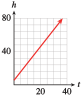
\includegraphics[width=\linewidth]{external/photos/fig-in-ex-ans-1-1-1.pdf}
\end{sbspanel}%
\end{sidebyside}%
\par
\end{inlineexercise}%
\begin{inlineexercise}{Practice 2.}{g:exercise:idp17}%
Use your equation from Practice 1 to answer the questions.  Illustrate each answer on the graph.%
\par
%
\begin{enumerate}[label=\alph*.]
\item{}How tall is the corn after 3 weeks? Use ``ft'' for feet or ``in'' for inches.%
\par
Answer (including units): \fillin{3.636363636363636}%
\item{}How long will it be before the corn is 6 feet tall? Use ``day'' for days.%
\par
Answer (including units): \fillin{3.636363636363636}%
\end{enumerate}
%
\par\smallskip%
\noindent\textbf{\blocktitlefont Answer 1}.\hypertarget{g:answer:idp18}{}\quad{}\(48\ {\rm in}\)%
\par\smallskip%
\noindent\textbf{\blocktitlefont Answer 2}.\hypertarget{g:answer:idp19}{}\quad{}\(33\ {\rm day}\)%
\par\smallskip%
\noindent\textbf{\blocktitlefont Solution}.\hypertarget{g:solution:idp20}{}\quad{}%
\begin{enumerate}[label=\alph*.]
\item{}48 inches tall%
\item{}33 days%
\end{enumerate}
%
\par
A graph is below.%
\par\medskip\noindent The graph below illustrates the answers.%
\begin{sidebyside}{1}{0}{0.75}{0}%
\begin{sbspanel}{0.25}%
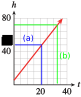
\includegraphics[width=\linewidth]{external/photos/fig-in-ex-ans-1-1-2.pdf}
\end{sbspanel}%
\end{sidebyside}%
\par
\end{inlineexercise}%
\begin{inlineexercise}{Pause and Reflect.}{g:exercise:idp21}%
What is the difference between an expression and an equation?%
\end{inlineexercise}%
\end{subsectionptx}
%
%
\typeout{************************************************}
\typeout{Subsection  Choosing Scales for the Axes}
\typeout{************************************************}
%
\begin{subsectionptx}{Choosing Scales for the Axes}{}{Choosing Scales for the Axes}{}{}{g:subsection:idp22}
To create a useful graph, we must choose appropriate scales for the axes.%
\par
%
\begin{itemize}[label=\textbullet]
\item{}The axes must extend far enough to show the values of the variables.%
\item{}The tick marks should be equally spaced.%
\item{}Usually we should use no more than 10 or 15 tick marks.%
\end{itemize}
%
\begin{example}{}{x:example:example-home-price}%
In 1990, the median price of a home in the US was \textdollar{}92,000.  The median price increased by about \textdollar{}4700 per year over the next decade.%
\begin{enumerate}[label=\alph*]
\item{}Make a table of values showing the median price of a house in 1990, 1994, 1998, and 2000.%
\item{}Choose suitable scales for the axes and plot the values you found in part (a) on a graph. Use \(t\), the number of years since 1990, on the horizontal axis and the price of the house, \(P\), on the vertical axis.  Draw a curve through the points.%
\item{}Write an equation that expresses \(P\) in terms of \(t\).%
\item{}How much did the price of the house increase from 1990 to 1996?  Illustrate the increase on your graph.%
\end{enumerate}
%
\par\smallskip%
\noindent\textbf{\blocktitlefont Solution}.\hypertarget{g:solution:idp23}{}\quad{}%
\begin{enumerate}[label=\alph*]
\item{}In 1990 the median price was \textdollar{}92,000.  Four years later, in 1994, the price had increased by \(\alert{4}(4700)=18,800\) dollars, so%
\begin{equation*}
P=92,000+\alert{4}(4700)=110,800
\end{equation*}
In 1998 the price had increased by \(\alert{8}(4700)=37,600\)  dollars, so%
\begin{equation*}
P=92,000+\alert{8}(4700)=129,600
\end{equation*}
You can verify the price of the house in 2000 by a similar calculation.%
\begin{center}%
{\tabularfont%
\begin{tabular}{AcAcAcA}\hrulethick
Year&Price of House)&\((t,P)\)\tabularnewline\hrulethin
\(1990\)&\(92,000\)&\((0,\, 92,000)\)\tabularnewline\hrulethin
\(1994\)&\(110,800\)&\((4,\, 110,800)\)\tabularnewline\hrulethin
\(1998\)&\(129,600\)&\((8,\, 129,600)\)\tabularnewline\hrulethin
\(2000\)&\(139,000\)&\((10,\, 139,000)\)\tabularnewline\hrulethin
\end{tabular}
}%
\end{center}%
\item{}We let \(t\) stand for the number of years since 1990, so that \(t=0\) in 1990, \(t=4\) in 1994, and so on.  To choose scales for the axes, we look at the values in the table.  For this graph we scale the horizontal axis, or \(t\)-axis, in 1-year intervals and the vertical axis, or \(P\)-axis, for \textdollar{}90,000 to \textdollar{}140,000 in intervals of \textdollar{}5,000. The points lie on a straight line, as shown in the figure.%
\begin{sidebyside}{1}{0.3}{0.3}{0}%
\begin{sbspanel}{0.4}%
\includegraphics[width=\linewidth]{external/photos/fig1-3.pdf}
\end{sbspanel}%
\end{sidebyside}%
\item{}Look back at the calculations in part (a).  The price of the house started at \textdollar{}92,000 in 1990 and increased by \(t \times 4700\) dollars after \(t\) years.  Thus,%
\begin{equation*}
P=92,000+4700t
\end{equation*}
%
\item{}We find the points on the graph for 1990 and 1996. These points lie above \(t=0\) and \(t=6\) on the \(t\)-axis.  Next we find the values on the \(P\)-axis corresponding to the two points.  The values are \(P=92,000\) in 1990 and \(P=120,200\) in 1996.  The increase in price is the difference of the two \(P\)-values.%
\begin{align*}
\text{increase in price}\amp=120,200-92,000\\
\amp=28,200
\end{align*}
The price of the home increased \textdollar{}28,200 between 1990 and 1996.  This increase is indicated by the arrows in the figure.%
\end{enumerate}
%
\end{example}
\begin{inlineexercise}{QuickCheck 2.}{g:exercise:idp24}%
If \(C\) is expressed in terms of \(H\text{,}\) which variable goes on the horizontal axis?%
\par
\begin{itemize}[label=$\odot$,leftmargin=3em,]
\item{}\(\displaystyle C\)%

\item{}\(\displaystyle H\)%

\item{}\(\displaystyle x\)%

\item{}The smaller one%

\end{itemize}
%
\par\smallskip%
\noindent\textbf{\blocktitlefont Answer}.\hypertarget{g:answer:idp25}{}\quad{}\(\text{Choice 2}\)%
\par\smallskip%
\noindent\textbf{\blocktitlefont Solution}.\hypertarget{g:solution:idp26}{}\quad{}\(H\)%
\end{inlineexercise}%
\begin{note}{}{g:note:idp27}%
The graphs in the preceding examples are \terminology{increasing graphs} \index{increasing graphs}.  As we move along the graph from left to right (in the direction of increasing \(t\) ), the second coordinate increases as well.  Try \hyperref[x:exercise:exercise-Silver-Lake]{Checkpoint~{\xreffont\ref{x:exercise:exercise-Silver-Lake}}}, which illustrates a \terminology{decreasing graph}\index{decreasing graph}.%
\end{note}
\begin{inlineexercise}{Practice 3.}{x:exercise:exercise-Silver-Lake}%
Silver Lake has been polluted by industrial waste products. The concentration of toxic chemicals in the water is currently 285 parts per million (ppm). Environmental officials would like to reduce the concentration by 15 ppm each year.%
\par
%
\begin{enumerate}[label=\alph*.]
\item{}Complete the table of values showing the desired concentration, \(C\text{,}\) of toxic chemicals \(t\) years from now. For each \(t\)-value, calculate the corresponding value for \(C\text{.}\)  Write your answers as ordered pairs.%
\begin{sidebyside}{1}{0}{0}{0}%
\begin{sbspanel}{1}%
\resizebox{\linewidth}{!}{%
{\centering%
{\tabularfont%
\begin{tabular}{llll}
\(t\)&\(C\)&&\((t,C)\)\tabularnewline[0pt]
\(0\)&&\(C=285-15(\alert{0})\)&(0, \fillin{1.363636363636364} )\tabularnewline[0pt]
\(5\)&&\(C=285-15(\alert{5})\)&(5, \fillin{1.363636363636364} )\tabularnewline[0pt]
\(10\)&&\(C=285-15(\alert{10})\)&(10, \fillin{1.363636363636364} )\tabularnewline[0pt]
\(15\)&&\(C=285-15(\alert{15})\)&(15, \fillin{1.363636363636364} )
\end{tabular}
}%
\par}
}%
\end{sbspanel}%
\end{sidebyside}%
\item{}To choose scales for the axes, notice that the value of \(C\) starts at 285 and decreases from there. We'll scale the vertical axis up to 300, and use 10 tick marks at intervals of 30. Graph the ordered pairs on the grid, and connect them with a straight line.%
\item{}Write an equation for the concentration, \(C\text{,}\)  of toxic chemicals \(t\) years from now.%
\par
Equation: \fillin{9.090909090909092}%
\end{enumerate}
%
\par\smallskip%
\noindent\textbf{\blocktitlefont Hint}.\hypertarget{g:hint:idp28}{}\quad{}For part (c): The concentration is initially 285 ppm, and we subtract 15 ppm for each year that passes, or \(15 \times t\text{.}\)%
\par\smallskip%
\noindent\textbf{\blocktitlefont Answer 1}.\hypertarget{g:answer:idp29}{}\quad{}\(285\)%
\par\smallskip%
\noindent\textbf{\blocktitlefont Answer 2}.\hypertarget{g:answer:idp30}{}\quad{}\(210\)%
\par\smallskip%
\noindent\textbf{\blocktitlefont Answer 3}.\hypertarget{g:answer:idp31}{}\quad{}\(135\)%
\par\smallskip%
\noindent\textbf{\blocktitlefont Answer 4}.\hypertarget{g:answer:idp32}{}\quad{}\(60\)%
\par\smallskip%
\noindent\textbf{\blocktitlefont Answer 5}.\hypertarget{g:answer:idp33}{}\quad{}\(C+15t = 285\)%
\par\smallskip%
\noindent\textbf{\blocktitlefont Solution}.\hypertarget{g:solution:idp34}{}\quad{}%
\begin{enumerate}[label=\alph*.]
\item{}\begin{sidebyside}{1}{0}{0}{0}%
\begin{sbspanel}{1}%
\resizebox{\linewidth}{!}{%
{\centering%
{\tabularfont%
\begin{tabular}{l}
\((t,C)\)\tabularnewline[0pt]
\((0,285)\)\tabularnewline[0pt]
\((5,210)\)\tabularnewline[0pt]
\((10,135)\)\tabularnewline[0pt]
\((15,60)\)
\end{tabular}
}%
\par}
}%
\end{sbspanel}%
\end{sidebyside}%
%
\item{}The graph is shown below.%
\item{}\(\displaystyle C=285-15t\)%
\end{enumerate}
%
\par\medskip\noindent The graph for part(b):%
\begin{sidebyside}{1}{0.35}{0.35}{0}%
\begin{sbspanel}{0.3}%
\includegraphics[width=\linewidth]{external/photos/fig-in-ex-ans-1-1-3.pdf}
\end{sbspanel}%
\end{sidebyside}%
\par
\end{inlineexercise}%
\begin{note}{}{g:note:idp35}%
In the previous Exercise, we extend the graph until it reaches the horizontal axis, but no farther.  Points with negative \(C\)-coordinates have no meaning for the problem.%
\end{note}
\begin{inlineexercise}{QuickCheck 3.}{g:exercise:idp36}%
If \(x \gt 5\text{,}\) what is true about \(-2x\text{?}\)%
\par
\begin{itemize}[label=$\odot$,leftmargin=3em,]
\item{}It is greater than 3%

\item{}It is less than 3%

\item{}It is greater than 10%

\item{}It is less than -10%

\end{itemize}
%
\par\smallskip%
\noindent\textbf{\blocktitlefont Answer}.\hypertarget{g:answer:idp37}{}\quad{}\(\text{It is less than -10}\)%
\par\smallskip%
\noindent\textbf{\blocktitlefont Solution}.\hypertarget{g:solution:idp38}{}\quad{}\(-2x\) is less than \(-10\text{.}\)%
\end{inlineexercise}%
\begin{technology}{Graphing an Equation.}{g:technology:idp39}%
We can use a graphing utililty to graph an equation. On most utilities, we follow three steps.%
\par
To Graph an Equation:%
\par
%
\begin{enumerate}
\item{}Press \kbd{Y=} and enter the equation you wish to graph.%
\item{}Press \kbd{WINDOW} and select a suitable graphing window.%
\item{}Press \kbd{GRAPH}%
\end{enumerate}
%
\end{technology}
\begin{example}{Using a Graphing Utility.}{x:example:graphing-calculator}%
In \hyperref[x:example:example-home-price]{Example~{\xreffont\ref{x:example:example-home-price}}}, we found the equation%
\begin{equation*}
P = 92,000 + 4700t
\end{equation*}
for the median price of a house \(t\) years after 1990. Graph this equation with technology.%
\par\smallskip%
\noindent\textbf{\blocktitlefont Solution}.\hypertarget{g:solution:idp40}{}\quad{}To begin, we press \kbd{Y=} and enter%
\begin{equation*}
Y1 = 92,000 + 4700X
\end{equation*}
%
\par
For this graph, we’ll use the grid in \hyperref[x:example:example-home-price]{Example~{\xreffont\ref{x:example:example-home-price}}} for our window settings, so we press \kbd{WINDOW} and enter%
\begin{center}%
{\tabularfont%
\begin{tabular}{lll}
Xmin\(=0\)&&Xmax\(=10\)\tabularnewline[0pt]
Ymin\(=90,000\)&&Ymax\(=140,000\)
\end{tabular}
}%
\end{center}%
Finally, we press \kbd{GRAPH}. The graph is shown in the figure.%
\begin{sidebyside}{1}{0.3}{0.3}{0}%
\begin{sbspanel}{0.4}%
\includegraphics[width=\linewidth]{external/photos/fig-GC-house-price.pdf}
\end{sbspanel}%
\end{sidebyside}%
\end{example}
\begin{inlineexercise}{Practice 4.}{g:exercise:idp41}%
%
\begin{enumerate}[label=\alph*.]
\item{}Solve the equation \(2y-1575=45x\) for \(y\) in terms of \(x\text{.}\)%
\par
\(y=\)\fillin{4.545454545454546}%
\item{}Graph the equation with a graphing utility. Use the window%
\begin{sidebyside}{1}{0}{0}{0}%
\begin{sbspanel}{1}%
\resizebox{\linewidth}{!}{%
{\centering%
{\tabularfont%
\begin{tabular}{lllll}
Xmin\(=-50\)&&Xmax\(=50\)&&Xscl\(=5\)\tabularnewline[0pt]
Ymin\(=-500\)&&Ymax\(=1000\)&&Yscl\(=100\)
\end{tabular}
}%
\par}
}%
\end{sbspanel}%
\end{sidebyside}%
\item{}Sketch the graph on paper. Use the window settings to choose appropriate scales for the axes.%
\end{enumerate}
%
\par\smallskip%
\noindent\textbf{\blocktitlefont Answer}.\hypertarget{g:answer:idp42}{}\quad{}\(\frac{1575+45x}{2}\)%
\par\smallskip%
\noindent\textbf{\blocktitlefont Solution}.\hypertarget{g:solution:idp43}{}\quad{}%
\begin{enumerate}[label=\alph*.]
\item{}\(\displaystyle y=(1575+45x)/2\)%
\item{}The calculator graph is shown below.%
\item{}The graph is shown below.%
\end{enumerate}
%
\par\medskip\noindent The graph for (b):%
\begin{sidebyside}{1}{0.05}{0.6}{0}%
\begin{sbspanel}{0.3}%
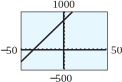
\includegraphics[width=\linewidth]{external/photos/fig-in-ex-ans-1-1-4b.pdf}
\end{sbspanel}%
\end{sidebyside}%
\par
c.%
\begin{sidebyside}{1}{0.05}{0.65}{0}%
\begin{sbspanel}{0.25}%
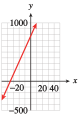
\includegraphics[width=\linewidth]{external/photos/fig-in-ex-ans-1-1-4c.pdf}
\end{sbspanel}%
\end{sidebyside}%
\par
\end{inlineexercise}%
\begin{inlineexercise}{QuickCheck 4.}{g:exercise:idp44}%
\begin{sidebyside}{1}{0.3}{0.3}{0}%
\begin{sbspanel}{0.4}%
\resizebox{\linewidth}{!}{%
\tikzset{%
}
\begin{tikzpicture} [scale=.8]
\draw[cyan] (0,0) grid (5,5);
\draw[black,thick,->,>=stealth'] (0,0)--(5.8,0);
\draw[black,thick,->,>=stealth'] (0,0)--(0,5.6);

\draw[black, thick] (1,0.14) --++(0,-.28) node[below, yshift=-2, fill=white, inner sep=1, scale=.9] {$5$};
\draw[black, thick] (2,0.14) --++(0,-.28) node[below, yshift=-2, fill=white, inner sep=1, scale=.9] {$20$};
\draw[black, thick] (3,0.14) --++(0,-.28) node[below, yshift=-2, fill=white, inner sep=1, scale=.9] {$30$};
\draw[black, thick] (4,0.14) --++(0,-.28) node[below, yshift=-2, fill=white, inner sep=1, scale=.9] {$50$};
\draw[black, thick] (5,0.14) --++(0,-.28) node[below, yshift=-2, fill=white, inner sep=1, scale=.9] {$100$};


\draw[black, thick] (0.14,1) --++(-.28,0) node[left, xshift=-2, fill=white, inner sep=1, scale=.9] {$20$};
\draw[black, thick] (0.14,2) --++(-.28,0) node[left, xshift=-2, fill=white, inner sep=1, scale=.9] {$25$};
\draw[black, thick] (0.14,3) --++(-.28,0) node[left, xshift=-2, fill=white, inner sep=1, scale=.9] {$30$};
\draw[black, thick] (0.14,4) --++(-.28,0) node[left, xshift=-2, fill=white, inner sep=1, scale=.9] {$35$};
\draw[black, thick] (0.14,5) --++(-.28,0) node[left, xshift=-2, fill=white, inner sep=1, scale=.9] {$40$};
\end{tikzpicture}
}%
\end{sbspanel}%
\end{sidebyside}%
\par\medskip
What is wrong with the grid above?%
\par
\begin{itemize}[label=$\odot$,leftmargin=3em,]
\item{}The grid lines on the \(x\)-axis are not evenly spaced.%

\item{}The scale on the \(y\)-axis does not start at 0.%

\item{}The axes are not labeled with the variables.%

\item{}All of the above.%

\end{itemize}
%
\par\smallskip%
\noindent\textbf{\blocktitlefont Answer}.\hypertarget{g:answer:idp45}{}\quad{}\(\text{Choice 4}\)%
\end{inlineexercise}%
\end{subsectionptx}
%
%
\typeout{************************************************}
\typeout{Subsection  Linear Equations}
\typeout{************************************************}
%
\begin{subsectionptx}{Linear Equations}{}{Linear Equations}{}{}{g:subsection:idp46}
All the models in the preceding examples have equations with a similar form:%
\begin{equation*}
\blert{y=\text{(starting value)}+\text{(rate of change)}\cdot x}
\end{equation*}
(We'll talk more about rate of change in \mono{[cross-reference to target(s) \textquotedbl{}slope-and-rate-of-change\textquotedbl{} missing or not unique]}.)  Their graphs were all portions of straight lines.  For this reason such equations are called  \terminology{linear equations}\index{linear equations}.  The order of the terms in the equation does not matter.  For example, the equation in \hyperref[x:example:example-Annelise]{Example~{\xreffont\ref{x:example:example-Annelise}}},%
\begin{equation*}
C=5+3t
\end{equation*}
can be written equivalently as%
\begin{equation*}
-3t+C=5
\end{equation*}
and the equation in \hyperref[x:example:example-home-price]{Example~{\xreffont\ref{x:example:example-home-price}}},%
\begin{equation*}
P=92,000+4700t
\end{equation*}
can be written as%
\begin{equation*}
-4700t +P=92,000
\end{equation*}
This form of a linear equation, \(Ax+By=C \), is called the \terminology{general form}\index{general form}.%
\begin{assemblage}{General Form for a Linear Equation.}{g:assemblage:idp47}%
The graph of any equation%
\begin{equation*}
Ax+By=C
\end{equation*}
where \(A\) and \(B\) are not both equal to zero, is a straight line.%
\end{assemblage}
\begin{example}{}{x:example:example-advertising}%
The manager at Albert's Appliances has \textdollar{}3000 to spend on advertising for the next fiscal quarter.  A 30-second spot on television costs \textdollar{}150 per broadcast, and a 30-second radio ad costs \textdollar{}50.%
\par
%
\begin{enumerate}[label=\alph*]
\item{}The manager decides to buy \(x\) television ads and \(y\) radio ads.  Write an equation relating \(x\) and \(y\).%
\item{}Make a table of values showing several choices for \(x\) and \(y\).%
\item{}Plot the points from your table, and graph the equation.%
\end{enumerate}
%
\par\smallskip%
\noindent\textbf{\blocktitlefont Solution}.\hypertarget{g:solution:idp48}{}\quad{}%
\begin{enumerate}[label=\alph*]
\item{}Each television ad costs \textdollar{}150, so \(x\) ads will cost \textdollar{}\(150x\).  Similarly, \(y\) radio ads will cost \textdollar{}\(50y\).  The manager has \textdollar{}3000 to spend, so the sum of the costs must be \textdollar{}3000.  Thus,%
\begin{equation*}
150x+50y=3000
\end{equation*}
%
\item{}We choose some values of \(x\), and solve the equation for the corresponding value of \(y\).  For example, if \(x=\alert{10}\) then%
\begin{align*}
150(\alert{10})+50y\amp=300\\
1500+50y\amp=3000\\
50y\amp=1500\\
y\amp=30
\end{align*}
If the manager buys 10 television ads, she can also buy 30 radio ads.  You can verify the other entries in the table.%
\begin{center}%
{\tabularfont%
\begin{tabular}{AcAcAcAcAcA}\hrulethick
\(x\)&\(8\)&\(10\)&\(12\)&\(14\)\tabularnewline\hrulethin
\(y\)&\(36\)&\(30\)&\(24\)&\(18\)\tabularnewline\hrulethin
\end{tabular}
}%
\end{center}%
\item{}\begin{sidebyside}{2}{0}{0.02}{0.18}%
\begin{sbspanel}{0.5}%
We plot the points from the table. All the solutions lie on a straight line, as shown in the figure.%
\end{sbspanel}%
\begin{sbspanel}{0.3}%
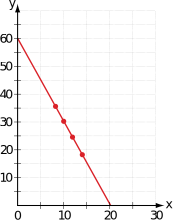
\includegraphics[width=\linewidth]{external/photos/fig-example-advertising.pdf}
\end{sbspanel}%
\end{sidebyside}%
%
\end{enumerate}
%
\end{example}
\begin{inlineexercise}{Practice 5.}{x:exercise:exercise-crops}%
In central Nebraska, each acre of corn requires 25 acre-inches of water per year, and each acre of winter wheat requires 18 acre-inches of water. (An acre-inch is the amount of water needed to cover one acre of land to a depth of one inch.) A farmer can count on 9000 acre-inches of water for the coming year. (Source: Institute of Agriculture and Natural Resources, University of Nebraska)%
\par
%
\begin{enumerate}[label=\alph*.]
\item{}Write an equation relating the number of acres of corn, \(x\text{,}\)  and the number of acres of wheat, \(y\text{,}\)  that the farmer can plant.%
\item{}Complete the table. Round your answers to tenths.%
\begin{sidebyside}{1}{0}{0}{0}%
\begin{sbspanel}{1}%
\resizebox{\linewidth}{!}{%
{\centering%
{\tabularfont%
\begin{tabular}{lllll}
\(x\)&\(50\)&\(100\)&\(150\)&\(200\)\tabularnewline[0pt]
\(y\)&\fillin{1.818181818181818}&\fillin{1.818181818181818}&\fillin{1.818181818181818}&\fillin{1.818181818181818}
\end{tabular}
}%
\par}
}%
\end{sbspanel}%
\end{sidebyside}%
\end{enumerate}
%
\par\smallskip%
\noindent\textbf{\blocktitlefont Answer 1}.\hypertarget{g:answer:idp49}{}\quad{}\(25x+18y = 9000\)%
\par\smallskip%
\noindent\textbf{\blocktitlefont Answer 2}.\hypertarget{g:answer:idp50}{}\quad{}\(430.556\)%
\par\smallskip%
\noindent\textbf{\blocktitlefont Answer 3}.\hypertarget{g:answer:idp51}{}\quad{}\(361.111\)%
\par\smallskip%
\noindent\textbf{\blocktitlefont Answer 4}.\hypertarget{g:answer:idp52}{}\quad{}\(291.667\)%
\par\smallskip%
\noindent\textbf{\blocktitlefont Answer 5}.\hypertarget{g:answer:idp53}{}\quad{}\(222.222\)%
\par\smallskip%
\noindent\textbf{\blocktitlefont Solution}.\hypertarget{g:solution:idp54}{}\quad{}%
\begin{enumerate}[label=\alph*.]
\item{}\(\displaystyle 25x+18y=9000\)%
\item{}\begin{sidebyside}{1}{0}{0}{0}%
\begin{sbspanel}{1}%
\resizebox{\linewidth}{!}{%
{\centering%
{\tabularfont%
\begin{tabular}{lllll}
\(x\)&\(50\)&\(100\)&\(150\)&\(200\)\tabularnewline[0pt]
\(y\)&\(430.6\)&\(361.1\)&\(291.7\)&\(222.2\)
\end{tabular}
}%
\par}
}%
\end{sbspanel}%
\end{sidebyside}%
%
\end{enumerate}
%
\end{inlineexercise}%
\begin{inlineexercise}{Pause and Reflect.}{g:exercise:idp55}%
Write down two different equation forms for linear models.  Which do you think is easier to use?%
\end{inlineexercise}%
\end{subsectionptx}
%
%
\typeout{************************************************}
\typeout{Subsection  Intercepts}
\typeout{************************************************}
%
\begin{subsectionptx}{Intercepts}{}{Intercepts}{}{}{g:subsection:idp56}
\begin{sidebyside}{2}{0}{0}{0.05}%
\begin{sbspanel}{0.25}[center]%
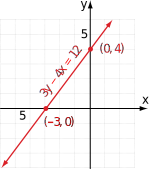
\includegraphics[width=\linewidth]{external/photos/fig-intercepts.pdf}
\end{sbspanel}%
\begin{sbspanel}{0.7}[center]%
Consider the graph of the equation%
\begin{equation*}
3x-4y=12
\end{equation*}
shown at left. The points where the graph crosses the axes are called the \terminology{intercepts}\index{intercept} of the graph. The coordinates of these points are easy to find.%
\end{sbspanel}%
\end{sidebyside}%
\par
The \(y\)-coordinate of the \(x\)-intercept is zero, so we set \(y=\alert{0}\) in the equation to get%
\begin{align*}
3(\alert{0})-4x\amp=12\\
x=-3
\end{align*}
%
\par
The \(x\)-intercept is the point \((-3,0)\). Also, the \(x\)-coordinate of the \(y\)-intercept is zero, so we set \(x=\alert{0}\) in the equation to get%
\begin{gather*}
3y-4(\alert{0})=12\\
y=4
\end{gather*}
The \(y\)-intercept is \((0,4)\).%
\begin{inlineexercise}{QuickCheck 5.}{g:exercise:idp57}%
What is the \(y\)-coordinate of any point on the \(x\)-axis?%
\par
\begin{itemize}[label=$\odot$,leftmargin=3em,]
\item{}\(\displaystyle (x,y)\)%

\item{}\(\displaystyle Y\)%

\item{}It depends on the value of \(x\)%

\item{}0%

\end{itemize}
%
\par\smallskip%
\noindent\textbf{\blocktitlefont Answer}.\hypertarget{g:answer:idp58}{}\quad{}\(\text{Choice 4}\)%
\par\smallskip%
\noindent\textbf{\blocktitlefont Solution}.\hypertarget{g:solution:idp59}{}\quad{}\(0\)%
\end{inlineexercise}%
\begin{assemblage}{Intercepts of a Graph.}{g:assemblage:idp60}%
The points where a graph crosses the axes are called the \terminology{intercepts of the graph}\index{intercept}.%
\begin{enumerate}
\item{}To find the \(y\)-intercept, set \(x=0\) and solve for \(y\).%
\item{}To find the \(x\)-intercept, set \(y=0\) and solve for \(x\)%
\end{enumerate}
%
\end{assemblage}
The intercepts of a graph tell us something about the situation it models.%
\begin{example}{}{x:example:example-intercepts}%
%
\begin{enumerate}[label=\alph*]
\item{}Find the intercepts of the graph in \hyperref[x:exercise:exercise-Silver-Lake]{Checkpoint~{\xreffont\ref{x:exercise:exercise-Silver-Lake}}}, about the pollution in Silver Lake.%
\item{}What do the intercepts tell us about the problem?%
\end{enumerate}
%
\par\smallskip%
\noindent\textbf{\blocktitlefont Solution}.\hypertarget{g:solution:idp61}{}\quad{}%
\begin{enumerate}[label=\alph*]
\item{}An equation for the concentration of toxic chemicals is%
\begin{equation*}
C=285-15t
\end{equation*}
To find the \(C\)-intercept, set \(t\) equal to zero.%
\begin{equation*}
C=285-15(\alert{0})=285
\end{equation*}
The \(C\)-intercept is the point \((0, 285)\), or simply 285.%
\par
To find the \(t\)-intercept, set \(C\) equal to zero and solve for \(t\).%
\par
%
\begin{equation*}
\begin{aligned}[t]
\alert{0}\amp =285-15t \amp \amp \blert{\text{Add }15t \text{ to both sides.}}\\
15t\amp =285  \amp \amp \blert{\text{Divide both sides by 15.}}\\
t\amp =19 
\end{aligned}
\end{equation*}
%
\par
The \(t\)-intercept is the point \((19,0)\), or simply \(19\).%
\item{}The \(C\)-intercept represents the concentration of toxic chemicals in Silver Lake now:  When  \(t=0\), \(C=285\),  so the concentration is currently \(285\) ppm.%
\par
The \(t\)-intercept represents the number of years it will take for the concentration of toxic chemicals to drop to zero:  When \(C=0\), \(t=19\),  so it will take \(19\) years for the pollution to be eliminated entirely.%
\end{enumerate}
%
\end{example}
\begin{inlineexercise}{QuickCheck 6.}{g:exercise:idp62}%
Delbert says that the intercepts of the line \(3x+5y=30\) are \((10,6)\text{.}\) What is wrong with his answer?%
\par
\begin{itemize}[label=$\odot$,leftmargin=3em,]
\item{}\((10,6)\) is not on the \(x\)-axis.%

\item{}An intercept must have a 0 coordinate.%

\item{}The line has two intercepts.%

\item{}All of the above%

\end{itemize}
%
\par\smallskip%
\noindent\textbf{\blocktitlefont Answer}.\hypertarget{g:answer:idp63}{}\quad{}\(\text{Choice 4}\)%
\par\smallskip%
\noindent\textbf{\blocktitlefont Solution}.\hypertarget{g:solution:idp64}{}\quad{}All of the above%
\end{inlineexercise}%
\begin{inlineexercise}{Practice 6.}{g:exercise:idp65}%
Find the intercepts of the graph in \hyperref[x:example:example-advertising]{Example~{\xreffont\ref{x:example:example-advertising}}}, about the advertising budget for Albert's Appliances: \(150x + 50y = 3000\).%
\par\medskip
%
\begin{enumerate}[label=\alph*.]
\item{}Enter each intercept as an ordered pair.%
\par
The \(x\)-intercept is \fillin{1.818181818181818}.%
\par
The \(y\)-intercept is \fillin{1.818181818181818}.%
\item{}What do the intercepts tell us about the problem?%
\par
The \(x\)-intercept tells us:%
\par
\begin{itemize}[label=$\odot$,leftmargin=3em,]
\item{}A) the cost of the TV ads.%

\item{}B) the best number of TV ads.%

\item{}C) the most TV ads she can buy for the money.%

\item{}D) the average number of TV ads.%

\end{itemize}
%
\par
The \(y\)-intercept tells us:%
\par
\begin{itemize}[label=$\odot$,leftmargin=3em,]
\item{}A) the cost of the radio ads.%

\item{}B) the number of radio ads she bought%

\item{}C) the number of radio ads if no TV ads are bought.%

\item{}D) the average cost per ad.%

\end{itemize}
%
\end{enumerate}
%
\par\smallskip%
\noindent\textbf{\blocktitlefont Answer 1}.\hypertarget{g:answer:idp66}{}\quad{}\(\left(20,0\right)\)%
\par\smallskip%
\noindent\textbf{\blocktitlefont Answer 2}.\hypertarget{g:answer:idp67}{}\quad{}\(\left(0,60\right)\)%
\par\smallskip%
\noindent\textbf{\blocktitlefont Answer 3}.\hypertarget{g:answer:idp68}{}\quad{}\(\text{C) the ... the money.}\)%
\par\smallskip%
\noindent\textbf{\blocktitlefont Answer 4}.\hypertarget{g:answer:idp69}{}\quad{}\(\text{C) the ... are bought.}\)%
\par\smallskip%
\noindent\textbf{\blocktitlefont Solution}.\hypertarget{g:solution:idp70}{}\quad{}%
\begin{enumerate}[label=\alph*.]
\item{}We find the \(x\)-intercept by setting \(y=0\) and solving for \(x\) to learn that \(x=20\text{,}\) so the \(x\)-intercept is \({\left(20,0\right)}\text{.}\)%
\par
We find the \(y\)-intercept by setting \(x=0\) and solving for \(y\) to learn that \(y=60\text{,}\) so the \(y\)-intercept is \({\left(0,60\right)}\text{.}\)%
\item{}The \(x\)-intercept has \(y=0\text{,}\) that is, it corresponds to when there are zero radio ads. The \(y\)-intercept has \(x=0\text{,}\) that is, it corresponds to when there are zero tv ads.%
\end{enumerate}
%
\end{inlineexercise}%
\begin{inlineexercise}{Pause and Reflect.}{g:exercise:idp71}%
Explain how the words intercept and intersect are related, and how they are different.%
\end{inlineexercise}%
\end{subsectionptx}
%
%
\typeout{************************************************}
\typeout{Subsection  Intercept Method for Graphing Lines}
\typeout{************************************************}
%
\begin{subsectionptx}{Intercept Method for Graphing Lines}{}{Intercept Method for Graphing Lines}{}{}{g:subsection:idp72}
Because we really only need two points to graph a linear equation, we might as well find the intercepts first and use them to draw the graph. The values of the intercepts will also help us choose suitable scales for the axes. It is always a good idea to find a third point as a check.%
\begin{example}{}{x:example:intercepts}%
%
\begin{enumerate}[label=\alph*]
\item{}Find the \(x\)- and \(y\)-intercepts of the graph of \(150x - 180y = 9000\).%
\item{}Use the intercepts to graph the equation. Find a third point as a check.%
\end{enumerate}
%
\par\smallskip%
\noindent\textbf{\blocktitlefont Solution}.\hypertarget{g:solution:idp73}{}\quad{}%
\begin{enumerate}[label=\alph*]
\item{}To find the \(x\)-intercept, we set \(y = \alert{0}\).%
\par
%
\begin{equation*}
\begin{aligned}[t]
150x-18(\alert{0})\amp =9000 \amp \amp \blert{\text{Simpify.}}\\
150x\amp =9000 \amp \amp \blert{\text{Divide both sides by 150.}}\\
x\amp =60   \amp \amp  
\end{aligned}
\end{equation*}
%
\par
The \(x\)-intercept is the point \((60, 0)\). To find the \(y\)-intercept, we set \(x = \alert{0}\).%
\par
%
\begin{equation*}
\begin{aligned}[t]
150(\alert{0})-18y\amp =9000 \amp \amp \blert{\text{Simpify.}}\\
-180y\amp =9000 \amp \amp \blert{\text{Divide both sides by } -180\text{.}}\\
y\amp =-50   \amp \amp  
\end{aligned}
\end{equation*}
%
\par
The \(y\)-intercept is the point \((0, -50)\).%
\item{}We scale both axes in intervals of 10 and then plot the two intercepts, \((60, 0)\) and \((0, -50)\). We draw the line through them, as shown below. Finally, we find another point and check that it lies on this line. We choose \(x = \alert{20}\) and solve for \(y\).%
\begin{align*}
150(\alert{20}) -180y \amp = 9000\\
3000 -180y \amp = 9000\\
-180y \amp = 6000\\
y \amp =-33.\overline{3}
\end{align*}
We plot the point \((20, -33\frac{1}{3})\). Because this point lies on the line, we can be reasonably confident that our graph is correct.%
\begin{sidebyside}{1}{0.35}{0.35}{0}%
\begin{sbspanel}{0.3}%
\includegraphics[width=\linewidth]{external/photos/fig-example-graph-intercepts.pdf}
\end{sbspanel}%
\end{sidebyside}%
\end{enumerate}
%
\end{example}
\begin{inlineexercise}{QuickCheck 7.}{g:exercise:idp74}%
Is it possible for the \(x\)-intercept and the \(y\)-intercept of a line to be the same point?%
\par
\begin{itemize}[label=$\odot$,leftmargin=3em,]
\item{}No%

\item{}Yes%

\item{}Only for a vertical line%

\item{}They are always the same point.%

\end{itemize}
%
\par\smallskip%
\noindent\textbf{\blocktitlefont Answer}.\hypertarget{g:answer:idp75}{}\quad{}\(\text{Yes}\)%
\par\smallskip%
\noindent\textbf{\blocktitlefont Solution}.\hypertarget{g:solution:idp76}{}\quad{}Yes%
\end{inlineexercise}%
\begin{assemblage}{To Graph a Line Using the Intercept Method:.}{g:assemblage:idp77}%
%
\begin{enumerate}[label=\arabic*]
\item{}Find the intercepts of the line.%
\begin{enumerate}[label=\alph*]
\item{}To find the \(x\)-intercept, set \(y=0\) and solve for \(x\).%
\item{}To find the \(y\)-intercept, set \(x=0\) and solve for \(y\).%
\end{enumerate}
%
\item{}Plot the intercepts.%
\item{}Choose a value for \(x\) and find a third point on the line.%
\item{}Draw a line through the points.%
\end{enumerate}
%
\end{assemblage}
\begin{inlineexercise}{QuickCheck 8.}{g:exercise:idp78}%
How many points do you need to graph a linear equation?%
\par
\begin{itemize}[label=$\odot$,leftmargin=3em,]
\item{}Two%

\item{}Three%

\item{}One in each quadrant%

\item{}It depends on the equation%

\end{itemize}
%
\par\smallskip%
\noindent\textbf{\blocktitlefont Answer}.\hypertarget{g:answer:idp79}{}\quad{}\(\text{Two}\)%
\par\smallskip%
\noindent\textbf{\blocktitlefont Solution}.\hypertarget{g:solution:idp80}{}\quad{}Two%
\end{inlineexercise}%
\begin{technology}{Choosing a Graphing Window.}{g:technology:idp81}%
Knowing the intercepts can also help us choose a suitable window on a graphing utility. We would like the window to be large enough to show the intercepts. For the graph in the example above, we can enter the equation%
\begin{equation*}
Y = (9000 -150X)/{-180}
\end{equation*}
in the window%
\begin{center}%
{\tabularfont%
\begin{tabular}{lll}
Xmin\(=-20\)&&Xmax\(=70\)\tabularnewline[0pt]
Ymin\(=-70\)&&Ymax\(=30\)
\end{tabular}
}%
\end{center}%
\end{technology}
\begin{inlineexercise}{Practice 7.}{g:exercise:idp82}%
In \hyperref[x:exercise:exercise-crops]{Checkpoint~{\xreffont\ref{x:exercise:exercise-crops}}} you wrote an equation about crops in Nebraska.%
\par\medskip
%
\begin{enumerate}[label=\alph*.]
\item{}Find the intercepts of the graph.%
\par
Note: Enter each intercept as an ordered pair.%
\par
The \(x\)-intercept is \fillin{2.727272727272727}.%
\par
The \(y\)-intercept is \fillin{2.727272727272727}.%
\item{}Use the intercepts to help you choose appropriate scales for the axes, and then graph the equation.%
\item{}What do the intercepts tell us about the problem?%
\par
The \(x\)-intercept tells us:%
\par
\begin{itemize}[label=$\odot$,leftmargin=3em,]
\item{}A) the total water usage of corn.%

\item{}B) the cost of the corn if no wheat is planted.%

\item{}C) the optimal number of acres of corn.%

\item{}D) the total acres if all corn is planted.%

\end{itemize}
%
\par
The \(y\)-intercept tells us:%
\par
\begin{itemize}[label=$\odot$,leftmargin=3em,]
\item{}A) the largest possible number of acres of wheat.%

\item{}B) the amount of water used by the wheat.%

\item{}C) the total cost of the wheat.%

\item{}D) how many acres are left after the wheat is planted.%

\end{itemize}
%
\end{enumerate}
%
\par\smallskip%
\noindent\textbf{\blocktitlefont Answer 1}.\hypertarget{g:answer:idp83}{}\quad{}\(\left(360,0\right)\)%
\par\smallskip%
\noindent\textbf{\blocktitlefont Answer 2}.\hypertarget{g:answer:idp84}{}\quad{}\(\left(0,500\right)\)%
\par\smallskip%
\noindent\textbf{\blocktitlefont Answer 3}.\hypertarget{g:answer:idp85}{}\quad{}\(\text{D) the ... is planted.}\)%
\par\smallskip%
\noindent\textbf{\blocktitlefont Answer 4}.\hypertarget{g:answer:idp86}{}\quad{}\(\text{A) the ... of wheat.}\)%
\par\smallskip%
\noindent\textbf{\blocktitlefont Solution}.\hypertarget{g:solution:idp87}{}\quad{}%
\begin{enumerate}[label=\alph*.]
\item{}We find the \(x\)-intercept by setting \(y=0\) and solving for \(x\) to learn that \(x=360\text{,}\) so the \(x\)-intercept is \({\left(360,0\right)}\text{.}\)%
\par
We find the \(y\)-intercept by setting \(x=0\) and solving for \(y\) to learn that \(y=500\text{,}\) so the \(y\)-intercept is \({\left(0,500\right)}\text{.}\)%
\item{}The \(x\)-intercept has \(y=0\text{,}\) that is, it corresponds to when there are zero radio ads. The \(y\)-intercept has \(x=0\text{,}\) that is, it corresponds to when there are zero tv ads.%
\end{enumerate}
%
\par\medskip\noindent A graph is shown below.%
\begin{sidebyside}{1}{0.375}{0.375}{0}%
\begin{sbspanel}{0.25}%
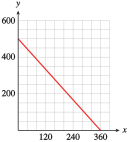
\includegraphics[width=\linewidth]{external/photos/fig-in-ex-ans-1-1-7.pdf}
\end{sbspanel}%
\end{sidebyside}%
\par
\end{inlineexercise}%
\begin{note}{}{g:note:idp88}%
The examples in this section model simple linear relationships between two variables. Such relationships, in which the value of one variable is determined by the value of the other, are called \terminology{functions}\index{function}. We will study various kinds of functions throughout the course.%
\end{note}
\begin{inlineexercise}{Pause and Reflect.}{g:exercise:idp89}%
What was the most difficult part of this section to understand? Write a question whose answer would help you understand it.%
\end{inlineexercise}%
\end{subsectionptx}
%
%
\typeout{************************************************}
\typeout{Subsection  Section Summary}
\typeout{************************************************}
%
\begin{subsectionptx}{Section Summary}{}{Section Summary}{}{}{x:subsection:summary-1-1}
%
%
\typeout{************************************************}
\typeout{Subsubsection  Vocabulary}
\typeout{************************************************}
%
\begin{subsubsectionptx}{Vocabulary}{}{Vocabulary}{}{}{g:subsubsection:idp90}
Look up the definitions of new terms in the Glossary.%
\begin{multicols}{3}
\begin{itemize}[label=\textbullet]
\item{}Variable%
\item{}Solve an equation%
\item{}Evaluate an expression%
\item{}Linear equation%
\item{}Increasing graph%
\item{}Decreasing graph%
\item{}Intercept%
\item{}Mathematical model%
\end{itemize}
\end{multicols}
%
\end{subsubsectionptx}
%
%
\typeout{************************************************}
\typeout{Subsubsection  CONCEPTS}
\typeout{************************************************}
%
\begin{subsubsectionptx}{CONCEPTS}{}{CONCEPTS}{}{}{g:subsubsection:idp91}
%
\begin{enumerate}[label=\arabic*]
\item{}We can describe a relationship between variables with a table of values, a graph, or an equation.%
\item{}Linear models have equations of the following form:%
\begin{equation*}
y = (\text{starting value}) + (\text{rate of change})\cdot x
\end{equation*}
%
\item{}To make a useful graph, we must choose appropriate scales for the axes.%
\item{}\begin{assemblage}{General Form for a Linear Equation.}{g:assemblage:idp92}%
The graph of any equation%
\begin{equation*}
Ax+By=C
\end{equation*}
where \(A\) and \(B\) are not both equal to zero, is a straight line.%
\end{assemblage}
%
\item{}The intercepts of a graph are the points where the graph crosses the axes.%
\item{}We can use the intercepts to graph a line.%
\par
%
\begin{assemblage}{To Graph a Line Using the Intercept Method:.}{g:assemblage:idp93}%
%
\begin{enumerate}[label=\arabic*]
\item{}Find the intercepts of the line.%
\begin{enumerate}[label=\alph*]
\item{}To find the \(x\)-intercept, set \(y=0\) and solve for \(x\).%
\item{}To find the \(y\)-intercept, set \(x=0\) and solve for \(y\).%
\end{enumerate}
%
\item{}Plot the intercepts.%
\item{}Choose a value for \(x\) and find a third point on the line.%
\item{}Draw a line through the points.%
\end{enumerate}
%
\end{assemblage}
\item{}The intercepts are also useful for interpreting a model.%
\end{enumerate}
%
\end{subsubsectionptx}
%
%
\typeout{************************************************}
\typeout{Subsubsection  STUDY QUESTIONS}
\typeout{************************************************}
%
\begin{subsubsectionptx}{STUDY QUESTIONS}{}{STUDY QUESTIONS}{}{}{g:subsubsection:idp94}
%
\begin{enumerate}[label=\arabic*]
\item{}Name three ways to represent a relationship between two variables.%
\item{}If \(C\) is expressed in terms of \(H\), which variable goes on the horizontal axis?%
\item{}Explain the difference between evaluating an expression and solving an equation.%
\item{}How many points do you need to graph a linear equation?%
\item{}Explain how the words \terminology{intercept} and \terminology{intersect} are related; explain how they are different.%
\item{}Delbert says that the intercepts of the line \(3x + 5y = 30\) are \((10, 6)\). What is wrong with his answer?%
\end{enumerate}
%
\end{subsubsectionptx}
%
%
\typeout{************************************************}
\typeout{Subsubsection  SKILLS}
\typeout{************************************************}
%
\begin{subsubsectionptx}{SKILLS}{}{SKILLS}{}{}{g:subsubsection:idp95}
Practice each skill in the Homework problems listed.%
\begin{enumerate}[label=\arabic*]
\item{}Make a table of values: \#1\textendash{}4, 7 and 8%
\item{}Plot points and draw a graph: \#1\textendash{}4, 7 and 8%
\item{}Choose appropriate scales for the axes: \#5\textendash{}12%
\item{}Write a linear model of the form \(y = (\text{starting value}) + (\text{rate of change})\cdot x\): \#1\textendash{}8%
\item{}Write a linear model in general form: \#25\textendash{}28, 33\textendash{}36%
\item{}Evaluate a linear expression, algebraically and graphically: \#1\textendash{}4%
\item{}Solve a linear equation, algebraically and graphically: \#1\textendash{}4%
\item{}Find the intercepts of a graph: \#5 and 6, 13\textendash{}24, 45\textendash{}52%
\item{}Graph a line by the intercept method: \#5 and 6, 13\textendash{}24%
\item{}Interpret the meaning of the intercepts: \#5 and 6, 25\textendash{}28%
\item{}Use a graphing calculator to graph a line: \#37\textendash{}52%
\item{}Sketch on paper a graph obtained on a calculator: \#37\textendash{}44%
\end{enumerate}
%
\end{subsubsectionptx}
\end{subsectionptx}
%
%
\typeout{************************************************}
\typeout{Exercises  Homework 1.1}
\typeout{************************************************}
%
\begin{exercises-subsection}{Homework 1.1}{}{Homework 1.1}{}{}{x:exercises:section-1-1-exercises}
\begin{divisionexercise}{1}{}{}{g:exercise:idp96}%
The temperature in the desert at 6 a.m., just before sunrise, was \(65\degree\)F. The temperature rose \(5\) degrees every hour until it reached its maximum value at about 5 p.m. Complete the table of values for the temperature, \(T\), at \(h\) hours after 6 a.m.%
\begin{center}%
{\tabularfont%
\begin{tabular}{AcAcAcAcAcAcA}\hrulethick
\(h\)&\(0\)&\(3\)&\(6\)&\(9\)&\(10\)\tabularnewline\hrulethin
\(T\)&\(\hphantom{0000}\)&\(\hphantom{0000}\)&\(\hphantom{0000}\)&\(\hphantom{0000}\)&\(\hphantom{0000}\)\tabularnewline\hrulethin
\end{tabular}
}%
\end{center}%
%
\begin{enumerate}[label=\alph*]
\item{}Write an equation for the temperature, \(T\), in terms of \(h\).%
\item{}Graph the equation.%
\begin{sidebyside}{1}{0.3}{0.3}{0}%
\begin{sbspanel}{0.4}%
\includegraphics[width=\linewidth]{external/photos/fig-ex-1-1-1.pdf}
\end{sbspanel}%
\end{sidebyside}%
\item{}How hot is it at noon? Illustrate the answer on your graph.%
\item{}When will the temperature be \(110\degree\)F? Illustrate the answer on your graph.%
\end{enumerate}
%
\end{divisionexercise}%
\begin{divisionexercise}{2}{}{}{g:exercise:idp97}%
The taxi out of Dulles Airport charges a traveler with one suitcase an initial fee of \textdollar{}\(2.00\), plus \textdollar{}\(1.50\) for each mile traveled. Complete the table of values showing the charge, \(C\), for a trip of \(n\) miles.%
\begin{center}%
{\tabularfont%
\begin{tabular}{AcAcAcAcAcAcAcA}\hrulethick
\(n\)&\(0\)&\(5\)&\(10\)&\(15\)&\(20\)&\(25\)\tabularnewline\hrulethin
\(C\)&\(\hphantom{0000}\)&\(\hphantom{0000}\)&\(\hphantom{0000}\)&\(\hphantom{0000}\)&\(\hphantom{0000}\)&\(\hphantom{0000}\)\tabularnewline\hrulethin
\end{tabular}
}%
\end{center}%
%
\begin{enumerate}[label=\alph*]
\item{}Write an equation for the charge, \(C\), in terms of the number of miles traveled, \(n\).%
\item{}Graph the equation.%
\begin{sidebyside}{1}{0.3}{0.3}{0}%
\begin{sbspanel}{0.4}%
\includegraphics[width=\linewidth]{external/photos/fig-ex-1-1-2.pdf}
\end{sbspanel}%
\end{sidebyside}%
\item{}What is the charge for a trip to Mount Vernon,  \(40\) miles from the airport? Illustrate the answer on your graph.%
\item{}If a ride to the National Institutes of Health (NIH) costs \textdollar{}\(39.50\), how far is it from the airport to the NIH? Illustrate the answer on your graph.%
\end{enumerate}
%
\end{divisionexercise}%
\begin{divisionexercise}{3}{}{}{g:exercise:idp98}%
On October 31, Betty and Paul fill their \(250\)-gallon oil tank for their heater. Beginning in November, they use an average of \(15\) gallons of oil per week. Complete the table of values for the amount of oil, \(A\), left in the tank after \(w\) weeks.%
\begin{center}%
{\tabularfont%
\begin{tabular}{AcAcAcAcAcAcA}\hrulethick
\(w\)&\(0\)&\(4\)&\(8\)&\(12\)&\(16\)\tabularnewline\hrulethin
\(A\)&\(\hphantom{0000}\)&\(\hphantom{0000}\)&\(\hphantom{0000}\)&\(\hphantom{0000}\)&\(\hphantom{0000}\)\tabularnewline\hrulethin
\end{tabular}
}%
\end{center}%
%
\begin{enumerate}[label=\alph*]
\item{}Write an equation that expresses the amount of oil, \(A\), in the tank in terms of the number of weeks, \(w\), since October 31.%
\item{}Graph the equation.%
\begin{sidebyside}{1}{0.3}{0.3}{0}%
\begin{sbspanel}{0.4}%
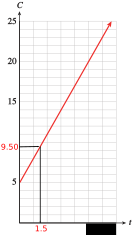
\includegraphics[width=\linewidth]{external/photos/fig-ex-1-1-3.pdf}
\end{sbspanel}%
\end{sidebyside}%
\item{}How much did the amount of fuel oil in the tank decrease between the third week and the eighth week? Illustrate this amount on the graph.%
\item{}When will the tank contain more than \(175\) gallons of fuel oil? Illustrate on the graph.%
\end{enumerate}
%
\end{divisionexercise}%
\begin{divisionexercise}{4}{}{}{g:exercise:idp99}%
Leon's camper has a \(20\)-gallon gas tank, and he gets \(12\) miles to the gallon. (That is, he uses \(\frac{1}{12}\) gallon per mile.) Complete the table of values for the amount of gas, \(g\), left in Leon's tank after driving \(m\) miles.%
\begin{center}%
{\tabularfont%
\begin{tabular}{AcAcAcAcAcAcA}\hrulethick
\(m\)&\(0\)&\(48\)&\(96\)&\(144\)&\(192\)\tabularnewline\hrulethin
\(g\)&\(\hphantom{0000}\)&\(\hphantom{0000}\)&\(\hphantom{0000}\)&\(\hphantom{0000}\)&\(\hphantom{0000}\)\tabularnewline\hrulethin
\end{tabular}
}%
\end{center}%
%
\begin{enumerate}[label=\alph*]
\item{}Write an equation that expresses the amount of gas, \(g\), in Leon's fuel tank in terms of the number of miles, \(m\), he has driven.%
\item{}Graph the equation.%
\begin{sidebyside}{1}{0.3}{0.3}{0}%
\begin{sbspanel}{0.4}%
\includegraphics[width=\linewidth]{external/photos/fig-ex-1-1-4.pdf}
\end{sbspanel}%
\end{sidebyside}%
\item{}How much gas will Leon use between 8 a.m., when his odometer reads \(96\) miles, and 9 a.m., when the odometer reads \(144\) miles? Illustrate on the graph.%
\item{}If Leon has less than \(5\) gallons of gas left, how many miles has he driven? Illustrate on the graph.%
\end{enumerate}
%
\end{divisionexercise}%
\begin{divisionexercise}{5}{}{}{g:exercise:idp100}%
Phil and Ernie buy a used photocopier for \textdollar{}\(800\) and set up a copy service on their campus. For each hour that the copier runs, Phil and Ernie make \textdollar{}\(40\).%
\begin{enumerate}[label=\alph*]
\item{}Write an equation that expresses Phil and Ernie's profit (or loss), \(P\), in terms of the number of hours, \(t\), they run the copier.%
\item{}Find the intercepts and sketch the graph. (Suggestion: Scale the horizontal axis from \(0\) to \(40\) in increments of \(5\), and scale the vertical axis from \(-1000\) to \(400\) in increments of \(100\).)%
\item{}What do the intercepts tell us about the profit?%
\end{enumerate}
%
\end{divisionexercise}%
\begin{divisionexercise}{6}{}{}{g:exercise:idp101}%
A deep-sea diver is taking some readings at a depth of \(400\) feet. He begins rising at \(20\) feet per minute.%
\begin{enumerate}[label=\alph*]
\item{}Write an equation that expresses the diver’s altitude, \(h\), in terms of the number of minutes, \(m\), elapsed. (Consider a depth of \(400\) feet as an altitude of \(-400\) feet.)%
\item{}Find the intercepts and sketch the graph. (Suggestion: Scale the horizontal axis from \(0\) to \(24\) in increments of \(2\), and scale the vertical axis from \(-500\) to \(100\) in increments of \(50\).)%
\item{}What do the intercepts tell us about the diver's depth?%
\end{enumerate}
%
\end{divisionexercise}%
\begin{divisionexercise}{7}{}{}{g:exercise:idp102}%
There are many formulas for estimating the annual cost of driving. The Automobile Club estimates that fixed costs for a small car—including insurance, registration, depreciation, and financing—total about \textdollar{}\(5000\) per year. The operating costs for gasoline, oil, maintenance, tires, and so forth are about \(12.5\) cents per mile. (Source: Automobile Association of America)%
\begin{enumerate}[label=\alph*]
\item{}Write an equation for the annual driving cost, \(C\), in terms of \(d\), the number of miles driven.%
\item{}Complete the table of values.%
\begin{center}%
{\tabularfont%
\begin{tabular}{AlAcAcAcAcAcA}\hrulethick
Miles Driven&\(4000\)&\(8000\)&\(12,000\)&\(16,000\)&\(20,000\)\tabularnewline\hrulethin
Cost (\textdollar{})&\(\hphantom{0000}\)&\(\hphantom{0000}\)&\(\hphantom{0000}\)&\(\hphantom{0000}\)&\(\hphantom{0000}\)\tabularnewline\hrulethin
\end{tabular}
}%
\end{center}%
\item{}Choose scales for the axes and graph the equation.%
\item{}How much does the annual cost of driving increase when the mileage increases from \(8000\) to \(12,000\) miles? Illustrate this amount on the graph.%
\item{}How much mileage will cause the annual cost to exceed \textdollar{}\(7000\)? Illustrate on the graph.%
\end{enumerate}
%
\end{divisionexercise}%
\begin{divisionexercise}{8}{}{}{g:exercise:idp103}%
The boiling point of water changes with altitude. At sea level, water boils at \(212\degree\)F, and the boiling point diminishes by approximately \(0.002\degree\)F for each \(1\)-foot increase in altitude.%
\begin{enumerate}[label=\alph*]
\item{}Write an equation for the boiling point, \(B\), in terms of \(a\), the altitude in feet.%
\item{}Complete the table of values.%
\begin{center}%
{\tabularfont%
\begin{tabular}{AlAcAcAcAcAcAcAcA}\hrulethick
Altitude (ft)&\(-500\)&\(0\)&\(1000\)&\(2000\)&\(3000\)&\(4000\)&\(5000\)\tabularnewline\hrulethin
Boiling point (\(\degree\)F)&\(\hphantom{0000}\)&\(\hphantom{0000}\)&\(\hphantom{0000}\)&\(\hphantom{0000}\)&\(\hphantom{0000}\)&\(\hphantom{0000}\)&\(\hphantom{0000}\)\tabularnewline\hrulethin
\end{tabular}
}%
\end{center}%
\item{}Choose scales for the axes and graph the equation.%
\item{}How much does the boiling point decrease when the altitude increases from \(1000\) to \(3000\) feet? Illustrate this amount on the graph.%
\item{}At what altitudes is the boiling point less than \(204\degree\)F? Illustrate on the graph.%
\end{enumerate}
%
\end{divisionexercise}%
\par\medskip\noindent%
\textbf{Exercise Group.}\space\space%
For each table, choose appropriate scales for the axes and plot the given points.%
\begin{exercisegroupcol}{2}
\begin{divisionexerciseegcol}{9}{}{}{g:exercise:idp104}%
\begin{center}%
{\tabularfont%
\begin{tabular}{AlAcAcAcAcA}\hrulethick
\(x\)&\(0\)&\(80\)&\(90\)&\(120\)\tabularnewline\hrulethin
\(y\)&\(6\)&\(2\)&\(1.5\)&\(1\)\tabularnewline\hrulethin
\end{tabular}
}%
\end{center}%
\end{divisionexerciseegcol}%
\begin{divisionexerciseegcol}{10}{}{}{g:exercise:idp105}%
\begin{center}%
{\tabularfont%
\begin{tabular}{AlAcAcAcAcA}\hrulethick
\(x\)&\(300\)&\(500\)&\(800\)&\(1100\)\tabularnewline\hrulethin
\(y\)&\(1.2\)&\(1.3\)&\(1.5\)&\(1.9\)\tabularnewline\hrulethin
\end{tabular}
}%
\end{center}%
\end{divisionexerciseegcol}%
\begin{divisionexerciseegcol}{11}{}{}{g:exercise:idp106}%
\begin{center}%
{\tabularfont%
\begin{tabular}{AlAcAcAcAcA}\hrulethick
\(x\)&\(0.01\)&\(0.03\)&\(0.06\)&\(0.07\)\tabularnewline\hrulethin
\(y\)&\(-0.2\)&\(-1\)&\(-1.1\)&\(-2\)\tabularnewline\hrulethin
\end{tabular}
}%
\end{center}%
\end{divisionexerciseegcol}%
\begin{divisionexerciseegcol}{12}{}{}{g:exercise:idp107}%
\begin{center}%
{\tabularfont%
\begin{tabular}{AlAcAcAcAcA}\hrulethick
\(x\)&\(0.003\)&\(0.005\)&\(0.008\)&\(0.011\)\tabularnewline\hrulethin
\(y\)&\(6\)&\(2\)&\(1.5\)&\(1\)\tabularnewline\hrulethin
\end{tabular}
}%
\end{center}%
\end{divisionexerciseegcol}%
\end{exercisegroupcol}
\par\medskip\noindent
\par\medskip\noindent%
\textbf{Exercise Group.}\space\space%
For Problems 13\textendash{}18,%
\begin{enumerate}[label=(\alph*)]
\item{}Find the intercepts of the graph.%
\item{}Graph the equation by the intercept method.%
\end{enumerate}
%
\begin{exercisegroupcol}{2}
\begin{divisionexerciseegcol}{13}{}{}{g:exercise:idp108}%
\(x + 2y = 8\)%
\end{divisionexerciseegcol}%
\begin{divisionexerciseegcol}{14}{}{}{g:exercise:idp109}%
\(2x - y = 6\)%
\end{divisionexerciseegcol}%
\begin{divisionexerciseegcol}{15}{}{}{g:exercise:idp110}%
\(3x - 4y =12\)%
\end{divisionexerciseegcol}%
\begin{divisionexerciseegcol}{16}{}{}{g:exercise:idp111}%
\(2x + 6y = 6\)%
\end{divisionexerciseegcol}%
\begin{divisionexerciseegcol}{17}{}{}{g:exercise:idp112}%
\(\displaystyle{\frac{x}{9}- \frac{y}{4}= 1}\)%
\end{divisionexerciseegcol}%
\begin{divisionexerciseegcol}{18}{}{}{g:exercise:idp113}%
\(\displaystyle{\frac{x}{5}+ \frac{y}{8}= 1}\)%
\end{divisionexerciseegcol}%
\end{exercisegroupcol}
\par\medskip\noindent
\par\medskip\noindent%
\textbf{Exercise Group.}\space\space%
For Problems 19-24,%
\begin{enumerate}[label=(\alph*)]
\item{}Find the intercepts of the graph.%
\item{}Use the intercepts to choose scales for the axes, and then graph the equation by the intercept method.%
\end{enumerate}
%
\begin{exercisegroupcol}{2}
\begin{divisionexerciseegcol}{19}{}{}{g:exercise:idp114}%
\(20x = 30y - 45,000\)%
\end{divisionexerciseegcol}%
\begin{divisionexerciseegcol}{20}{}{}{g:exercise:idp115}%
\(30x = 45y + 60,000\)%
\end{divisionexerciseegcol}%
\begin{divisionexerciseegcol}{21}{}{}{g:exercise:idp116}%
\(0.4x + 1.2y = 4.8\)%
\end{divisionexerciseegcol}%
\begin{divisionexerciseegcol}{22}{}{}{g:exercise:idp117}%
\(3.2x - 0.8y = 12.8\)%
\end{divisionexerciseegcol}%
\begin{divisionexerciseegcol}{23}{}{}{g:exercise:idp118}%
\(\displaystyle{\frac{2x}{3}+ \frac{3y}{11}= 1}\)%
\end{divisionexerciseegcol}%
\begin{divisionexerciseegcol}{24}{}{}{g:exercise:idp119}%
\(\displaystyle{\frac{8x}{7}- \frac{2y}{7}= 1}\)%
\end{divisionexerciseegcol}%
\end{exercisegroupcol}
\par\medskip\noindent
\begin{divisionexercise}{25}{}{}{g:exercise:idp120}%
The owner of a gas station has \textdollar{}\(19,200\) to spend on unleaded gas this month. Regular unleaded costs him \textdollar{}\(2.40\) per gallon, and premium unleaded costs \textdollar{}\(3.20\) per gallon.%
%
\begin{enumerate}[label=\alph*]
\item{}How much do \(x\) gallons of regular cost? How much do \(y\) gallons of premium cost?%
\item{}Write an equation in general form that relates the amount of regular unleaded gasoline, \(x\), the owner can buy and the amount of premium unleaded, \(y\).%
\item{}Find the intercepts and sketch the graph.%
\item{}What do the intercepts tell us about the amount of gasoline the owner can purchase?%
\end{enumerate}
\end{divisionexercise}%
\begin{divisionexercise}{26}{}{}{g:exercise:idp121}%
Five pounds of body fat is equivalent to \(16,000\) calories. Carol can burn \(600\) calories per hour bicycling and \(400\) calories per hour swimming.%
%
\begin{enumerate}[label=\alph*]
\item{}How many calories will Carol burn in \(x\) hours of cycling? How many calories will she burn in \(y\) hours of swimming?%
\item{}Write an equation in general form that relates the number of hours, \(x\), of cycling and the number of hours, \(y\), of swimming Carol needs to perform in order to lose \(5\) pounds.%
\item{}Find the intercepts and sketch the graph.%
\item{}What do the intercepts tell us about Carol's exercise program?%
\end{enumerate}
\end{divisionexercise}%
\begin{divisionexercise}{27}{}{}{g:exercise:idp122}%
Delbert must increase his daily potassium intake by \(1800\) mg. He decides to eat a combination of figs and bananas, which are both low in sodium. There are \(9\) mg potassium per gram of fig, and \(4\) mg potassium per gram of banana.%
%
\begin{enumerate}[label=\alph*]
\item{}How much potassium is in \(x\) grams of fig? How much potassium is in \(y\) grams of banana?%
\item{}Write an equation in general form that relates the number of grams, \(x\), of fig and the number of grams, \(y\), of banana Delbert needs to get \(1800\) mg of potassium.%
\item{}Find the intercepts and sketch the graph.%
\item{}What do the intercepts tell us about Delbert's diet?%
\end{enumerate}
\end{divisionexercise}%
\begin{divisionexercise}{28}{}{}{g:exercise:idp123}%
Leslie plans to invest some money in two CD accounts. The first account pays \(3.6\%\) interest per year, and the second account pays \(2.8\%\) interest per year. Leslie would like to earn \textdollar{}\(500\) per year on her investment.%
%
\begin{enumerate}[label=\alph*]
\item{}If Leslie invests \(x\) dollars in the first account, how much interest will she earn? How much interest will she earn if she invests \(y\) dollars in the second account?%
\item{}Write an equation in general form that relates \(x\) and \(y\) if Leslie earns \(\$500\) interest.%
\item{}Find the intercepts and sketch the graph.%
\item{}What do the intercepts tell us about Leslie's investments?%
\end{enumerate}
\end{divisionexercise}%
\begin{divisionexercise}{29}{}{}{g:exercise:idp124}%
Find the intercepts of the graph for each equation.%
%
\begin{multicols}{2}
\begin{enumerate}[label=\alph*]
\item{}\(\displaystyle \displaystyle{\frac{x}{3}+\frac{y}{5}=1} \)%
\item{}\(\displaystyle \displaystyle{2x - 4y = 1} \)%
\item{}\(\displaystyle \displaystyle{\frac{2x}{5}-\frac{2y}{3}=1} \)%
\item{}\(\displaystyle \displaystyle{\frac{x}{p}+\frac{y}{q}=1} \)%
\end{enumerate}
\end{multicols}
\(\hphantom{00}\) e.  Why is the equation \(\displaystyle{\frac{x}{a}+\frac{y}{b}=1} \) called the \terminology{intercept form} for a line?%
\end{divisionexercise}%
\begin{divisionexercise}{30}{}{}{g:exercise:idp125}%
Write an equation in intercept form (see Problem 29) for the line with the given intercepts. Then write the equation in general form.%
%
\begin{multicols}{2}
\begin{enumerate}[label=\alph*]
\item{}\(\displaystyle (6, 0), (0, 2) \)%
\item{}\(\displaystyle (-3, 0), (0, 8) \)%
\item{}\(\displaystyle \left(\dfrac{3}{4}, 0\right), \left(0, \dfrac{-1}{4}\right) \)%
\item{}\(\displaystyle (v, 0), (0, -w) \)%
\item{}\(\displaystyle \left(\dfrac{1}{H}, 0\right), \left(0, \dfrac{1}{T}\right) \)%
\end{enumerate}
\end{multicols}
\end{divisionexercise}%
\begin{divisionexercise}{31}{}{}{g:exercise:idp126}%
%
\begin{enumerate}[label=\alph*]
\item{}Find the \(y\)-intercept of the line \(y = mx + b\).%
\item{}Find the \(x\)-intercept of the line \(y = mx + b\).%
\end{enumerate}
%
\end{divisionexercise}%
\begin{divisionexercise}{32}{}{}{g:exercise:idp127}%
%
\begin{enumerate}[label=\alph*]
\item{}Find the \(y\)-intercept of the line \(Ax + By = C\).%
\item{}Find the \(x\)-intercept of the line \(Ax + By = C\).%
\end{enumerate}
%
\end{divisionexercise}%
\par\medskip\noindent%
\textbf{Exercise Group.}\space\space%
Write an equation in general form for each line.%
\begin{exercisegroupcol}{2}
\begin{divisionexerciseegcol}{33}{}{}{g:exercise:idp128}%
\begin{sidebyside}{1}{0.1}{0.1}{0}%
\begin{sbspanel}{0.8}%
\includegraphics[width=\linewidth]{external/photos/fig-ex-1-1-33.pdf}
\end{sbspanel}%
\end{sidebyside}%
\end{divisionexerciseegcol}%
\begin{divisionexerciseegcol}{34}{}{}{g:exercise:idp129}%
\begin{sidebyside}{1}{0.1}{0.1}{0}%
\begin{sbspanel}{0.8}%
\includegraphics[width=\linewidth]{external/photos/fig-ex-1-1-34.pdf}
\end{sbspanel}%
\end{sidebyside}%
\end{divisionexerciseegcol}%
\begin{divisionexerciseegcol}{35}{}{}{g:exercise:idp130}%
\begin{sidebyside}{1}{0.1}{0.1}{0}%
\begin{sbspanel}{0.8}%
\includegraphics[width=\linewidth]{external/photos/fig-ex-1-1-35.pdf}
\end{sbspanel}%
\end{sidebyside}%
\end{divisionexerciseegcol}%
\begin{divisionexerciseegcol}{36}{}{}{g:exercise:idp131}%
\begin{sidebyside}{1}{0.1}{0.1}{0}%
\begin{sbspanel}{0.8}%
\includegraphics[width=\linewidth]{external/photos/fig-ex-1-1-36.pdf}
\end{sbspanel}%
\end{sidebyside}%
\end{divisionexerciseegcol}%
\end{exercisegroupcol}
\par\medskip\noindent
\par\medskip\noindent%
\textbf{Exercise Group.}\space\space%
For Problems 37\textendash{}44,%
\begin{enumerate}[label=\alph*]
\item{}Solve each equation for \(y\) in terms of \(x\). (See the Algebra Skills Refresher \mono{[cross-reference to target(s) \textquotedbl{}appendix-Linear-Equations-and-Inequalities\textquotedbl{} missing or not unique]} to review this skill.)%
\item{}Graph the equation on your calculator in the specified window.%
\item{}Make a pencil and paper sketch of the graph. Label the scales on your axes, and the coordinates of the intercepts.%
\end{enumerate}
%
\begin{exercisegroupcol}{2}
\begin{divisionexerciseegcol}{37}{}{}{g:exercise:idp132}%
\(2+y=6\)%
\begin{align*}
{\text{Xmin}} \amp = -10 \amp\amp {\text{Ymin}} = -10\\
{\text{Xmax}} \amp = 10 \amp\amp {\text{Ymax}} = 10\\
{\text{Xscl}} \amp = 1 \amp\amp {\text{Yscl}} = 1
\end{align*}
%
\end{divisionexerciseegcol}%
\begin{divisionexerciseegcol}{38}{}{}{g:exercise:idp133}%
\(8 - y + 3x = 0\)%
\begin{align*}
{\text{Xmin}} \amp = -10 \amp\amp {\text{Ymin}} = -10\\
{\text{Xmax}} \amp = 10 \amp\amp {\text{Ymax}} = 10\\
{\text{Xscl}} \amp = 1 \amp\amp {\text{Yscl}} = 1
\end{align*}
%
\end{divisionexerciseegcol}%
\begin{divisionexerciseegcol}{39}{}{}{g:exercise:idp134}%
\(3x - 4y = 1200\)%
\begin{align*}
{\text{Xmin}} \amp = -1000 \amp\amp {\text{Ymin}} = -1000\\
{\text{Xmax}} \amp = 1000 \amp\amp {\text{Ymax}} = 1000\\
{\text{Xscl}} \amp = 100 \amp\amp {\text{Yscl}} = 100
\end{align*}
%
\end{divisionexerciseegcol}%
\begin{divisionexerciseegcol}{40}{}{}{g:exercise:idp135}%
\(x + 2y = 500\)%
\begin{align*}
{\text{Xmin}} \amp = -1000 \amp\amp {\text{Ymin}} = -1000\\
{\text{Xmax}} \amp = 1000 \amp\amp {\text{Ymax}} = 1000\\
{\text{Xscl}} \amp = 100 \amp\amp {\text{Yscl}} = 100
\end{align*}
%
\end{divisionexerciseegcol}%
\begin{divisionexerciseegcol}{41}{}{}{g:exercise:idp136}%
\(0.2x + 5y = 0.1\)%
\begin{align*}
{\text{Xmin}} \amp = -1 \amp\amp {\text{Ymin}} = -0.1\\
{\text{Xmax}} \amp = 1 \amp\amp {\text{Ymax}} = 0.1\\
{\text{Xscl}} \amp = 0.1 \amp\amp {\text{Yscl}} = 0.01
\end{align*}
%
\end{divisionexerciseegcol}%
\begin{divisionexerciseegcol}{42}{}{}{g:exercise:idp137}%
\(1.2x - 4.2y = 3.6\)%
\begin{align*}
{\text{Xmin}} \amp = -1 \amp\amp {\text{Ymin}} = -1\\
{\text{Xmax}} \amp = 4 \amp\amp {\text{Ymax}} = 1\\
{\text{Xscl}} \amp = 0.2 \amp\amp {\text{Yscl}} = 0.1
\end{align*}
%
\end{divisionexerciseegcol}%
\begin{divisionexerciseegcol}{43}{}{}{g:exercise:idp138}%
\(70x + 3y = y + 420\)%
\begin{align*}
{\text{Xmin}} \amp = 0 \amp\amp {\text{Ymin}} = 0\\
{\text{Xmax}} \amp = 10 \amp\amp {\text{Ymax}} = 250\\
{\text{Xscl}} \amp = 1 \amp\amp {\text{Yscl}} = 25
\end{align*}
%
\end{divisionexerciseegcol}%
\begin{divisionexerciseegcol}{44}{}{}{g:exercise:idp139}%
\(40y - 5x = 780 - 20y\)%
\begin{align*}
{\text{Xmin}} \amp = -200 \amp\amp {\text{Ymin}} = 0\\
{\text{Xmax}} \amp = 0 \amp\amp {\text{Ymax}} = 20\\
{\text{Xscl}} \amp = 20 \amp\amp {\text{Yscl}} = 2
\end{align*}
%
\end{divisionexerciseegcol}%
\end{exercisegroupcol}
\par\medskip\noindent
\par\medskip\noindent%
\textbf{Exercise Group.}\space\space%
For Problems 45\textendash{}52,%
\begin{enumerate}[label=\alph*]
\item{}Find the \(x\)- and \(y\)-intercepts.%
\item{}Solve the equation for \(y\).%
\item{}Choose a graphing window in which both intercepts are visible, and graph the equation on your calculator.%
\end{enumerate}
%
\begin{exercisegroupcol}{2}
\begin{divisionexerciseegcol}{45}{}{}{g:exercise:idp140}%
\(x + 4y = 100\)%
\end{divisionexerciseegcol}%
\begin{divisionexerciseegcol}{46}{}{}{g:exercise:idp141}%
\(2x - 3y = -72\)%
\end{divisionexerciseegcol}%
\begin{divisionexerciseegcol}{47}{}{}{g:exercise:idp142}%
\(25x - 20y = 1\)%
\end{divisionexerciseegcol}%
\begin{divisionexerciseegcol}{48}{}{}{g:exercise:idp143}%
\(4x + 75y = 60,000\)%
\end{divisionexerciseegcol}%
\begin{divisionexerciseegcol}{49}{}{}{g:exercise:idp144}%
\(\dfrac{y}{12} - \dfrac{x}{60}= 1\)%
\end{divisionexerciseegcol}%
\begin{divisionexerciseegcol}{50}{}{}{g:exercise:idp145}%
\(\dfrac{x}{80} + \dfrac{y}{400}= 1\)%
\end{divisionexerciseegcol}%
\begin{divisionexerciseegcol}{51}{}{}{g:exercise:idp146}%
\(-2x = 3y + 84\)%
\end{divisionexerciseegcol}%
\begin{divisionexerciseegcol}{52}{}{}{g:exercise:idp147}%
\(7x = 91 - 13y\)%
\end{divisionexerciseegcol}%
\end{exercisegroupcol}
\par\medskip\noindent
\end{exercises-subsection}
\end{sectionptx}
\end{chapterptx}
\end{document}